%%
%% This is file `monografia.tex'
%%

%%%%%%%%%%%%%%%%
%% Plantilla para la presentaci\'on de monograf\'ias de trabajo de grado
%% Carrera de Ingenier\'ia Electr\'onica
%% Pontificia Universidad Javeriana - Cali
%% Mayo 2020
%%%%%%%%%%%%%%%%

%\documentclass[11pt,twoside]{thesis-tg-ie-pujc}
\documentclass{thesis-tg-ie-pujc} % Se utiliza la nueva clase
\usepackage[utf8]{inputenc}
\usepackage{enumerate}
\usepackage{longtable}
\usepackage{xurl}
\usepackage[breaklinks]{hyperref}
\usepackage{makeidx}
\usepackage{multicol}
\usepackage{graphics}
\usepackage{pdflscape} % provides the landscape environment
\usepackage{ragged2e} % provides \RaggedLeft
\usepackage[intoc, spanish]{nomencl}
\usepackage[spanish]{babel}

%%%%%%%%%%%%%%%%%%
%%
%% This is file `author_data.tex'
%%

%%%%%%%%%%%%%%%%
%% Datos a modificar por los autores del proyecto de trabajo de grado
%% Carrera de Ingeniería Electrónica
%% Pontificia Universidad Javeriana – Cali
%% Julio 2025
%%%%%%%%%%%%%%%%

%%%%%%%%%%%%%%%%
% TÍTULO DEL PROYECTO
%%%%%%%%%%%%%%%%
\titulo
{Proyecto X}

%%%%%%%
% AUTOR
%%%%%%%
\autorA{8939280}{Juan José Restrepo Rosero}
\autorB{8992284}{María Valentina Belalcázar Perdomo}

%%%%%%%
% FECHA DE ENTREGA
%%%%%%%
\fecha{\today}

%%%%%%%%%%%%%%%%%
% METADATA PDF
% TÍTULO DEL TRABAJO DE GRADO
% AUTOR(ES)
% KEYWORDS
%%%%%%%%%%%%%%%%%
\hypersetup
{
  pdftitle={Proyecto X},
  pdfauthor={Juan José Restrepo Rosero, María Valentina Belalcázar Perdomo},
  pdfkeywords={Creación de Valor Compartido, Sostenibilidad, Pymes, Data Engineering, Multi-omics}
}

%%%%%%%%%%%%%%%%%
% DIRECTOR DEL PROYECTO
%%%%%%%%%%%%%%%%%
\directorproyecto{Dr.}{Julian Gil González}

%%%%%%%%%%%%%%%%%
% DECANO FACULTAD DE INGENIERÍA Y CIENCIAS
% DIRECTOR DE CARRERA
%%%%%%%%%%%%%%%%%
\decanoFIC{Dr.}{Hernán Camilo Rocha Niño}
\directorcarrera{Dr.}{Diego Luis Linares Ospina}

%%%%%%%
% VERSIÓN
%%%%%%%
\version{DEFINITIVA}

%%%%%%%
% JURADOS
%%%%%%%
\juradoA{Dr.}{Nombre Apellido} % Jurado 1
\juradoB{Dr.}{Nombre Apellido} % Jurado 2

\usepackage{changepage}
\usepackage[acronym]{glossaries}

%% Edited by colarte, Tek
\usepackage{ifthen}
\def\authorB{}
\def\authorBCOD{}
\def\codirector{}
%% end Colarte, Tek
\let\cleardoublepage=\clearpage
\NeedsTeXFormat{LaTeX2e}[1995/12/01]
\ProvidesClass{ThesisStyle}
              [2004/02/16 v1.4f
 Standard LaTeX document class]

%% Edited by Tek
\newcommand{\fecha}[1]{\def \fecha{#1}}
%Nombre del Trabajo
\newcommand{\titulo}[1]{\def \titulovar{#1}}
%Nombre del director del proyecto
\newcommand{\directorproyecto}[2]{\def \director{#1 #2}}
%Nombre del codirector del proyecto
%\newcommand{\codirectorproyecto}[2]{\def \codirector{#1 #2}}
%Nombre del director de carrera
\newcommand{\directorcarrera}[2]{\def \directorIE{#1 #2}}
%Autor(es)
\newcommand{\autorA}[2]{\def \authorA{#2}\def \authorACOD{#1}}
\newcommand{\autorB}[2]{\def \authorB{#2}\def \authorBCOD{#1}}
%\newcommand{\autorC}[2]{\def \authorC{#2}\def \authorCCOD{#1}}

%Decano
\newcommand{\decanoFIC}[2]{\def \deanFIC{#1 #2}}
%Jurados
\newcommand{\juradoA}[2]{\def \juryA{#1 #2}}
\newcommand{\juradoB}[2]{\def \juryB{#1 #2}}
%Version
\newcommand{\version}[1]{\def \versionvar{#1}}

\newcommand{\makecoverletter}
{


% % %%%%%%%%%% 2nd Letter - ACTA CORRECION %%%%%%%%%%%%%
% \thispagestyle{empty}
% %\ \newpage
% %\thispagestyle{empty}

% \noindent Santiago de Cali, \fecha
% \vskip 1cm
% \noindent \begin{center} \textbf{Acta de Correciones al Proyecto de Grado}\\
% \noindent Facultad de Ingenier\'ia y Ciencias \\
% \end{center}
% \vskip 1cm
% \noindent \textbf{Autores:} \authorA\, \authorB\ y \authorC\\
% \vskip 0.5cm
% \noindent \textbf{Proyecto:} ``\titulovar''\\

% \vskip 1cm
% \noindent Cordial Saludo.\\\\\\

% \ifthenelse{\equal{\codirector}{}}{Certifico,}{Certificamos,}
% como indica el artículo 2.27 de las Directrices de Trabajo de Grado, he verificado que los estudiantes indicados arriba han implementado todas las correcciones que los Jurados del Proyecto de Grado definieron que se efectuaran, como consta en el Acta de Calificación correspondiente.\\

% \noindent Atentamente,
% \vskip 3cm
% \ifthenelse{\equal{\codirector}{}}
% {
% \noindent \line(1,0){200}\\
% \noindent \director \\
% \noindent Director Trabajo de Grado
% }
% {\noindent
% \begin{tabular}{p{8cm}p{8cm}}
% \line(1,0){200}&\line(1,0){200} \\
% \director \\
% Director Trabajo de Grado
% \end{tabular}
% }


%%%%%%%%%% 1st Letter - aceptacion %%%%%%%%%%%%%
\ifthenelse{\equal{\versionvar}{DEFINITIVA}}
{
\thispagestyle{empty}
\ \newpage
\thispagestyle{empty}
\begin{adjustwidth}{8cm}{0.5cm}
\noindent Nota de Aceptación
\vskip 0.5cm
\noindent {Aprobado por el Comité de Trabajo de Grado en cumplimiento de los requisitos exigidos por la Pontificia Universidad Javeriana para optar al título de Magíster en Ciencia de Datos.}
\end{adjustwidth}
\vskip 3cm
\begin{center}
\line(1,0){200}\\
\deanFIC \\
Decano Facultad de Ingeniería y Ciencias \\
\vskip 2cm
\line(1,0){200}\\
\directorIE \\
Director Maestría en Ciencia de Datos \\
\vskip 2cm 
\ifthenelse{\equal{\codirector}{}}
{
\line(1,0){200}\\
\director \\
Director Trabajo de Grado
}
{
\begin{tabular}{c{8cm}c{8cm}}
\line(1,0){200}&\line(1,0){200} \\
\director \\
Director Trabajo de Grado \\
\end{tabular}
}
\vskip 2cm

\begin{tabular}{c{8cm}c{8cm}}
\line(1,0){200}&\line(1,0){200} \\
\juryA & \juryB\\
Jurado & Jurado\\
\end{tabular}
\end{center}
}

\cleardoublepage


%%%%%%%%%% 3th Letter - presentacion %%%%%%%%%%%%%

\thispagestyle{empty}
%\ \newpage
%\thispagestyle{empty}
\noindent Santiago de Cali, \fecha
\vskip 2cm
\noindent Se\~nores\\
\noindent {Pontificia Universidad Javeriana -- Cali}\\
\noindent \deanFIC \\
\noindent Decano \\
\noindent Facultad de Ingenier\'ia y Ciencias \\
\noindent Cali
\vskip 1.5cm
\noindent Cordial Saludo.\\\\\\
\ifthenelse{\value{numautores}=1}{Me permito}{Nos permitimos }% 
presentar a su consideración el Proyecto Aplicado titulado ``\titulovar'' con el fin de cumplir con los requisitos exigidos por la Universidad para llevar a cabo el proyecto de grado y posteriormente optar al título de Magíster en Ciencia de Datos.\\

Al firmar aquí,%
\ifthenelse{\value{numautores}=1}{ doy fe que entiendo y conozco}{ damos fe que entendemos y conocemos}%
 las directrices para la presentación de trabajos de grado de la Facultad de Ingeniería y Ciencias aprobadas el 26 de noviembre de 2009, donde se establecen los plazos y normas para el desarrollo del anteproyecto y del trabajo de grado.


\noindent Atentamente, \\[3cm]

\noindent
    \begin{tabular}{l}
    \line(1,0){200} \\
    \authorA \\
    Código: \authorACOD \\

    \\[2cm]
    \line(1,0){200} \\
    \authorB \\
    Código: \authorBCOD \\
\end{tabular}


\cleardoublepage

%%%%%%%%%% 4thrd Letter - certificacion %%%%%%%%%%%%%

\thispagestyle{empty}
\noindent Santiago de Cali, \fecha
\vskip 2cm
\noindent Se\~nores\\
\noindent {\bf Pontificia Universidad Javeriana -- Cali}\\
\noindent \deanFIC \\
\noindent Decano \\
\noindent Facultad de Ingenier\'ia y Ciencias \\
\noindent Cali
\vskip 2cm
\noindent Cordial Saludo.\\\\\\
Por medio de la presente me permito informarle que 
\ifthenelse{\value{numautores}=1}{el estudiante}{los estudiantes}%
 de la Maestría en Ciencia de Datos 
%
\ifthenelse{\value{numautores}=1}{%
  \authorA~(cod: \authorACOD) trabajó%
}{%
  \ifthenelse{\value{numautores}=2}{%
    \authorA~(cod: \authorACOD) y \authorB~(cod: \authorBCOD) trabajaron%
  }{%
    \authorA~(cod: \authorACOD) y \authorB~(cod: \authorBCOD) trabajaron %
  }%
}% 
 bajo mi dirección en el Proyecto Aplicado titulado `\titulovar'.\\\\\\




\noindent Atentamente,
\vskip 2cm
\ifthenelse{\equal{\codirector}{}}
{
\noindent \line(1,0){200}\\
\noindent \director \\
\noindent Director Trabajo de Grado
}
{\noindent
\begin{tabular}{p{8cm}p{8cm}}
\line(1,0){200}&\line(1,0){200} \\
\director
Director Trabajo de Grado 
\end{tabular}
}

\cleardoublepage
}
%% End: Edited by Tek

\newcommand\@ptsize{}
\newif\if@restonecol
\newif\if@titlepage
\@titlepagetrue
\newif\if@openright
\newif\if@mainmatter \@mainmattertrue
\if@compatibility\else
\DeclareOption{a4paper}
   {\setlength\paperheight {297mm}%
    \setlength\paperwidth  {210mm}}
\DeclareOption{a5paper}
   {\setlength\paperheight {210mm}%
    \setlength\paperwidth  {148mm}}
\DeclareOption{b5paper}
   {\setlength\paperheight {250mm}%
    \setlength\paperwidth  {176mm}}
\DeclareOption{letterpaper}
   {\setlength\paperheight {11in}%
    \setlength\paperwidth  {8.5in}}
\DeclareOption{legalpaper}
   {\setlength\paperheight {14in}%
    \setlength\paperwidth  {8.5in}}
\DeclareOption{executivepaper}
   {\setlength\paperheight {10.5in}%
    \setlength\paperwidth  {7.25in}}
\DeclareOption{landscape}
   {\setlength\@tempdima   {\paperheight}%
    \setlength\paperheight {\paperwidth}%
    \setlength\paperwidth  {\@tempdima}}
\fi
\if@compatibility
  \renewcommand\@ptsize{0}
\else
\DeclareOption{10pt}{\renewcommand\@ptsize{0}}
\fi
\DeclareOption{11pt}{\renewcommand\@ptsize{1}}
\DeclareOption{12pt}{\renewcommand\@ptsize{2}}
\if@compatibility\else
\DeclareOption{oneside}{\@twosidefalse \@mparswitchfalse}
\fi
\DeclareOption{twoside}{\@twosidetrue  \@mparswitchtrue}
\DeclareOption{draft}{\setlength\overfullrule{5pt}}
\if@compatibility\else
\DeclareOption{final}{\setlength\overfullrule{0pt}}
\fi
\DeclareOption{titlepage}{\@titlepagetrue}
\if@compatibility\else
\DeclareOption{notitlepage}{\@titlepagefalse}
\fi
\if@compatibility
\@openrighttrue
\else
\DeclareOption{openright}{\@openrighttrue}
\DeclareOption{openany}{\@openrightfalse}
\fi
\if@compatibility\else
\DeclareOption{onecolumn}{\@twocolumnfalse}
\fi
\DeclareOption{twocolumn}{\@twocolumntrue}
\DeclareOption{leqno}{\input{leqno.clo}}
\DeclareOption{fleqn}{\input{fleqn.clo}}
\DeclareOption{openbib}{%
  \AtEndOfPackage{%
   \renewcommand\@openbib@code{%
      \advance\leftmargin\bibindent
      \itemindent -\bibindent
      \listparindent \itemindent
      \parsep \z@
      }%
   \renewcommand\newblock{\par}}%
}
\ExecuteOptions{letterpaper,10pt,twoside,onecolumn,final,openright}
\ProcessOptions
\input{bk1\@ptsize.clo}
\setlength\lineskip{1\p@}
\setlength\normallineskip{1\p@}
\renewcommand\baselinestretch{}
\setlength\parskip{0\p@ \@plus \p@}
\@lowpenalty   51
\@medpenalty  151
\@highpenalty 301
\setcounter{topnumber}{2}
\renewcommand\topfraction{.7}
\setcounter{bottomnumber}{1}
\renewcommand\bottomfraction{.3}
\setcounter{totalnumber}{3}
\renewcommand\textfraction{.2}
\renewcommand\floatpagefraction{.5}
\setcounter{dbltopnumber}{2}
\renewcommand\dbltopfraction{.7}
\renewcommand\dblfloatpagefraction{.5}
\if@twoside
  \def\ps@headings{%
      \let\@oddfoot\@empty\let\@evenfoot\@empty
      \def\@evenhead{\thepage\hfil\slshape\leftmark}%
      \def\@oddhead{{\slshape\rightmark}\hfil\thepage}%
      \let\@mkboth\markboth
    \def\chaptermark##1{%
      \markboth {\MakeUppercase{%
        \ifnum \c@secnumdepth >\m@ne
          \if@mainmatter
            \@chapapp\ \thechapter. \ %
          \fi
        \fi
        ##1}}{}}%
    \def\sectionmark##1{%
      \markright {\MakeUppercase{%
        \ifnum \c@secnumdepth >\z@
          \thesection. \ %
        \fi
        ##1}}}}
\else
  \def\ps@headings{%
    \let\@oddfoot\@empty
    \def\@oddhead{{\slshape\rightmark}\hfil\thepage}%
    \let\@mkboth\markboth
    \def\chaptermark##1{%
      \markright {\MakeUppercase{%
        \ifnum \c@secnumdepth >\m@ne
          \if@mainmatter
            \@chapapp\ \thechapter. \ %
          \fi
        \fi
        ##1}}}}
\fi
\def\ps@myheadings{%
    \let\@oddfoot\@empty\let\@evenfoot\@empty
    \def\@evenhead{\thepage\hfil\slshape\leftmark}%
    \def\@oddhead{{\slshape\rightmark}\hfil\thepage}%
    \let\@mkboth\@gobbletwo
    \let\chaptermark\@gobble
    \let\sectionmark\@gobble
    }
  \if@titlepage
    % portada
    % Edited by C. Olarte, Tek
  \newcommand\maketitle{
  \begin{titlepage}%
      \let\footnotesize\small
      \let\footnoterule\relax
      \let \footnote \thanks
      \null\vfil
      \begin{center}
        Pontificia Universidad Javeriana Cali\\
        Facultad de Ingenier\'ia y Ciencias\\
        Maestría en Ciencia de Datos\\
        Proyecto Aplicado III
    \end{center}
    \vspace{2cm}
    \begin{center}%
        {\LARGE \titulovar \par}%
        \vskip 3em%
        {\large
        \lineskip .75em%
        \begin{tabular}[t]{c}%
        \authorA \\
        \authorB \\
        \\\\
        \\\\
        Director: \director
        \end{tabular}\par}%
        \vskip 1.5em%
        \vspace{1cm}
        {\large \fecha \par}%       % Set date in \large size.
        \end{center}\par
        \@thanks
        \vfil\null
        \begin{center}
        %
\includegraphics[width=8cm]{images/pujlogo.png}
        
\includegraphics[width=11cm,  height=3.5cm]{images/LogoPUJC.png}
      \end{center}
      \@thanks
      \vfil\null
  \end{titlepage}%
  \setcounter{footnote}{0}%
  \global\let\thanks\relax
  \global\let\maketitle\relax
  \global\let\@thanks\@empty
  \global\let\@author\@empty
  \global\let\@date\@empty
  \global\let\@title\@empty
  \global\let\title\relax
  \global\let\author\relax
  \global\let\date\relax
  \global\let\and\relax
}
\else
\newcommand\maketitle{\par
  \begingroup
    \renewcommand\thefootnote{\@fnsymbol\c@footnote}%
    \def\@makefnmark{\rlap{\@textsuperscript{\normalfont\@thefnmark}}}%
    \long\def\@makefntext##1{\parindent 1em\noindent
            \hb@xt@1.8em{%
                \hss\@textsuperscript{\normalfont\@thefnmark}}##1}%
    \if@twocolumn
      \ifnum \col@number=\@ne
        \@maketitle
      \else
        \twocolumn[\@maketitle]%
      \fi
    \else
      \newpage
      \global\@topnum\z@   % Prevents figures from going at top of page.
      \@maketitle
    \fi
    \thispagestyle{plain}\@thanks
  \endgroup
  \setcounter{footnote}{0}%
  \global\let\thanks\relax
  \global\let\maketitle\relax
  \global\let\@maketitle\relax
  \global\let\@thanks\@empty
  \global\let\@author\@empty
  \global\let\@date\@empty
  \global\let\@title\@empty
  \global\let\title\relax
  \global\let\author\relax
  \global\let\date\relax
  \global\let\and\relax
}
\def\@maketitle{%
  \newpage
  \null
  \vskip 2em%
  \begin{center}%
  \let \footnote \thanks
    {\LARGE \@title \par}%
    \vskip 1.5em%
    {\large
      \lineskip .5em%
      \begin{tabular}[t]{c}%
        \@author
      \end{tabular}\par}%
    \vskip 1em%
    {\large \@date}%
  \end{center}%
  \par
  \vskip 1.5em}
\fi
\newcommand*\chaptermark[1]{}
\setcounter{secnumdepth}{2}
\newcounter {part}
\newcounter {chapter}
\newcounter {section}[chapter]
\newcounter {subsection}[section]
\newcounter {subsubsection}[subsection]
\newcounter {paragraph}[subsubsection]
\newcounter {subparagraph}[paragraph]
\renewcommand \thepart {\@Roman\c@part}
\renewcommand \thechapter {\@arabic\c@chapter}
\renewcommand \thesection {\thechapter.\@arabic\c@section}
\renewcommand\thesubsection   {\thesection.\@arabic\c@subsection}
\renewcommand\thesubsubsection{\thesubsection .\@arabic\c@subsubsection}
\renewcommand\theparagraph    {\thesubsubsection.\@arabic\c@paragraph}
\renewcommand\thesubparagraph {\theparagraph.\@arabic\c@subparagraph}
\newcommand\@chapapp{\chaptername}
\newcommand\frontmatter{%
    \cleardoublepage
  \@mainmatterfalse
  \pagenumbering{roman}}
\newcommand\mainmatter{%
    \cleardoublepage
  \@mainmattertrue
  \pagenumbering{arabic}}
\newcommand\backmatter{%
  \if@openright
    \cleardoublepage
  \else
    \clearpage
  \fi
  \@mainmatterfalse}
\newcommand\part{%
  \if@openright
    \cleardoublepage
  \else
    \clearpage
  \fi
  \thispagestyle{plain}%
  \if@twocolumn
    \onecolumn
    \@tempswatrue
  \else
    \@tempswafalse
  \fi
  \null\vfil
  \secdef\@part\@spart}

\def\@part[#1]#2{%
    \ifnum \c@secnumdepth >-2\relax
      \refstepcounter{part}%
      \addcontentsline{toc}{part}{\thepart\hspace{1em}#1}%
    \else
      \addcontentsline{toc}{part}{#1}%
    \fi
    \markboth{}{}%
    {\centering
     \interlinepenalty \@M
     \normalfont
     \ifnum \c@secnumdepth >-2\relax
       \huge\bfseries \partname\nobreakspace\thepart
       \par
       \vskip 20\p@
     \fi
     \Huge \bfseries #2\par}%
    \@endpart}
\def\@spart#1{%
    {\centering
     \interlinepenalty \@M
     \normalfont
     \Huge \bfseries #1\par}%
    \@endpart}
\def\@endpart{\vfil\newpage
              \if@twoside
               \if@openright
                \null
                \thispagestyle{empty}%
                \newpage
               \fi
              \fi
              \if@tempswa
                \twocolumn
              \fi}
\newcommand\chapter{\if@openright\cleardoublepage\else\clearpage\fi
                    \thispagestyle{plain}%
                    \global\@topnum\z@
                    \@afterindentfalse
                    \secdef\@chapter\@schapter}
\def\@chapter[#1]#2{\ifnum \c@secnumdepth >\m@ne
                       \if@mainmatter
                         \refstepcounter{chapter}%
                         \typeout{\@chapapp\space\thechapter.}%
                         \addcontentsline{toc}{chapter}%
                                   {\protect\numberline{\thechapter}#1}%
                       \else
                         \addcontentsline{toc}{chapter}{#1}%
                       \fi
                    \else
                      \addcontentsline{toc}{chapter}{#1}%
                    \fi
                    \chaptermark{#1}%
                    \addtocontents{lof}{\protect\addvspace{10\p@}}%
                    \addtocontents{lot}{\protect\addvspace{10\p@}}%
                    \if@twocolumn
                      \@topnewpage[\@makechapterhead{#2}]%
                    \else
                      \@makechapterhead{#2}%
                      \@afterheading
                    \fi}

\def\@makechapterhead#1{%
%  \vspace*{10\p@}%
  {\parindent \z@ \raggedright \normalfont
    \begin{flushright}
      \ifnum \c@secnumdepth >\m@ne
        \if@mainmatter
%          \huge\bfseries 
          {\Large \scshape \@chapapp\space \thechapter}
          \par\nobreak
%        \vskip 0\p@
        \fi
      \fi
      \interlinepenalty\@M
      \Huge \bfseries #1\par\nobreak
      \hrulefill
    \end{flushright}
    \vskip 20\p@
  }}
\def\@schapter#1{\if@twocolumn
                   \@topnewpage[\@makeschapterhead{#1}]%
                 \else
                   \@makeschapterhead{#1}%
                   \@afterheading
                 \fi}
\def\@makeschapterhead#1{%
%  \vspace*{10\p@}%
  {\parindent \z@ \raggedright
    \normalfont
    \interlinepenalty\@M
    \begin{flushright}
	\Huge \bfseries  #1\par\nobreak
    \end{flushright}
    \vskip 20\p@
  }}
\newcommand\section{\@startsection {section}{1}{\z@}%
                                   {-3.5ex \@plus -1ex \@minus -.2ex}%
                                   {2.3ex \@plus.2ex}%
                                   {\normalfont\Large\bfseries}}
\newcommand\subsection{\@startsection{subsection}{2}{\z@}%
                                     {-3.25ex\@plus -1ex \@minus -.2ex}%
                                     {1.5ex \@plus .2ex}%
                                     {\normalfont\large\bfseries}}
\newcommand\subsubsection{\@startsection{subsubsection}{3}{\z@}%
                                     {-3.25ex\@plus -1ex \@minus -.2ex}%
                                     {1.5ex \@plus .2ex}%
                                     {\normalfont\normalsize\bfseries}}
\newcommand\paragraph{\@startsection{paragraph}{4}{\z@}%
                                    {3.25ex \@plus1ex \@minus.2ex}%
                                    {-1em}%
                                    {\normalfont\normalsize\bfseries}}
\newcommand\subparagraph{\@startsection{subparagraph}{5}{\parindent}%
                                       {3.25ex \@plus1ex \@minus .2ex}%
                                       {-1em}%
                                      {\normalfont\normalsize\bfseries}}
\if@twocolumn
  \setlength\leftmargini  {2em}
\else
  \setlength\leftmargini  {2.5em}
\fi
\leftmargin  \leftmargini
\setlength\leftmarginii  {2.2em}
\setlength\leftmarginiii {1.87em}
\setlength\leftmarginiv  {1.7em}
\if@twocolumn
  \setlength\leftmarginv  {.5em}
  \setlength\leftmarginvi {.5em}
\else
  \setlength\leftmarginv  {1em}
  \setlength\leftmarginvi {1em}
\fi
\setlength  \labelsep  {.5em}
\setlength  \labelwidth{\leftmargini}
\addtolength\labelwidth{-\labelsep}
\@beginparpenalty -\@lowpenalty
\@endparpenalty   -\@lowpenalty
\@itempenalty     -\@lowpenalty
\renewcommand\theenumi{\@arabic\c@enumi}
\renewcommand\theenumii{\@alph\c@enumii}
\renewcommand\theenumiii{\@roman\c@enumiii}
\renewcommand\theenumiv{\@Alph\c@enumiv}
\newcommand\labelenumi{\theenumi.}
\newcommand\labelenumii{(\theenumii)}
\newcommand\labelenumiii{\theenumiii.}
\newcommand\labelenumiv{\theenumiv.}
\renewcommand\p@enumii{\theenumi}
\renewcommand\p@enumiii{\theenumi(\theenumii)}
\renewcommand\p@enumiv{\p@enumiii\theenumiii}
\newcommand\labelitemi{\textbullet}
\newcommand\labelitemii{\normalfont\bfseries \textendash}
\newcommand\labelitemiii{\textasteriskcentered}
\newcommand\labelitemiv{\textperiodcentered}
\newenvironment{description}
               {\list{}{\labelwidth\z@ \itemindent-\leftmargin
                        \let\makelabel\descriptionlabel}}
               {\endlist}
\newcommand*\descriptionlabel[1]{\hspace\labelsep
                                \normalfont\bfseries #1}
\newenvironment{verse}
               {\let\\\@centercr
                \list{}{\itemsep      \z@
                        \itemindent   -1.5em%
                        \listparindent\itemindent
                        \rightmargin  \leftmargin
                        \advance\leftmargin 1.5em}%
                \item\relax}
               {\endlist}
\newenvironment{quotation}
               {\list{}{\listparindent 1.5em%
                        \itemindent    \listparindent
                        \rightmargin   \leftmargin
                        \parsep        \z@ \@plus\p@}%
                \item\relax}
               {\endlist}
\newenvironment{quote}
               {\list{}{\rightmargin\leftmargin}%
                \item\relax}
               {\endlist}
\if@compatibility
\newenvironment{titlepage}
    {%
      \cleardoublepage
      \if@twocolumn
        \@restonecoltrue\onecolumn
      \else
        \@restonecolfalse\newpage
      \fi
      \thispagestyle{empty}%
      \setcounter{page}\z@
    }%
    {\if@restonecol\twocolumn \else \newpage \fi
    }
\else
\newenvironment{titlepage}
    {%
      \cleardoublepage
      \if@twocolumn
        \@restonecoltrue\onecolumn
      \else
        \@restonecolfalse\newpage
      \fi
      \thispagestyle{empty}%
      \setcounter{page}\@ne
    }%
    {\if@restonecol\twocolumn \else \newpage \fi
     \if@twoside\else
        \setcounter{page}\@ne
     \fi
    }
\fi
\newcommand\appendix{\par
  \setcounter{chapter}{0}%
  \setcounter{section}{0}%
  \gdef\@chapapp{\appendixname}%
  \gdef\thechapter{\@Alph\c@chapter}}
\setlength\arraycolsep{5\p@}
\setlength\tabcolsep{6\p@}
\setlength\arrayrulewidth{.4\p@}
\setlength\doublerulesep{2\p@}
\setlength\tabbingsep{\labelsep}
\skip\@mpfootins = \skip\footins
\setlength\fboxsep{3\p@}
\setlength\fboxrule{.4\p@}
\@addtoreset {equation}{chapter}
\renewcommand\theequation
  {\ifnum \c@chapter>\z@ \thechapter.\fi \@arabic\c@equation}
\newcounter{figure}[chapter]
\renewcommand \thefigure
     {\ifnum \c@chapter>\z@ \thechapter.\fi \@arabic\c@figure}
\def\fps@figure{tbp}
\def\ftype@figure{1}
\def\ext@figure{lof}
\def\fnum@figure{\figurename\nobreakspace\thefigure}
\newenvironment{figure}
               {\@float{figure}}
               {\end@float}
\newenvironment{figure*}
               {\@dblfloat{figure}}
               {\end@dblfloat}
\newcounter{table}[chapter]
\renewcommand \thetable
     {\ifnum \c@chapter>\z@ \thechapter.\fi \@arabic\c@table}
\def\fps@table{tbp}
\def\ftype@table{2}
\def\ext@table{lot}
\def\fnum@table{\tablename\nobreakspace\thetable}
\newenvironment{table}
               {\@float{table}}
               {\end@float}
\newenvironment{table*}
               {\@dblfloat{table}}
               {\end@dblfloat}
\newlength\abovecaptionskip
\newlength\belowcaptionskip
\setlength\abovecaptionskip{10\p@}
\setlength\belowcaptionskip{0\p@}
\long\def\@makecaption#1#2{%
  \vskip\abovecaptionskip
  \sbox\@tempboxa{#1: #2}%
  \ifdim \wd\@tempboxa >\hsize
    #1: #2\par
  \else
    \global \@minipagefalse
    \hb@xt@\hsize{\hfil\box\@tempboxa\hfil}%
  \fi
  \vskip\belowcaptionskip}
\DeclareOldFontCommand{\rm}{\normalfont\rmfamily}{\mathrm}
\DeclareOldFontCommand{\sf}{\normalfont\sffamily}{\mathsf}
\DeclareOldFontCommand{\tt}{\normalfont\ttfamily}{\mathtt}
\DeclareOldFontCommand{\bf}{\normalfont\bfseries}{\mathbf}
\DeclareOldFontCommand{\it}{\normalfont\itshape}{\mathit}
\DeclareOldFontCommand{\sl}{\normalfont\slshape}{\@nomath\sl}
\DeclareOldFontCommand{\sc}{\normalfont\scshape}{\@nomath\sc}
\DeclareRobustCommand*\cal{\@fontswitch\relax\mathcal}
\DeclareRobustCommand*\mit{\@fontswitch\relax\mathnormal}
\newcommand\@pnumwidth{1.55em}
\newcommand\@tocrmarg{2.55em}
\newcommand\@dotsep{4.5}
\setcounter{tocdepth}{2}
\newcommand\tableofcontents{%
    \if@twocolumn
      \@restonecoltrue\onecolumn
    \else
      \@restonecolfalse
    \fi
    \chapter*{\contentsname
        \@mkboth{%
           \MakeUppercase\contentsname}{\MakeUppercase\contentsname}}%
	\@starttoc{toc}%
    \if@restonecol\twocolumn\fi
    }
\newcommand*\l@part[2]{%
  \ifnum \c@tocdepth >-2\relax
    \addpenalty{-\@highpenalty}%
    \addvspace{2.25em \@plus\p@}%
    \setlength\@tempdima{3em}%
    \begingroup
      \parindent \z@ \rightskip \@pnumwidth
      \parfillskip -\@pnumwidth
      {\leavevmode
       \large \bfseries #1\hfil \hb@xt@\@pnumwidth{\hss #2}}\par
       \nobreak
         \global\@nobreaktrue
         \everypar{\global\@nobreakfalse\everypar{}}%
    \endgroup
  \fi}
\newcommand*\l@chapter[2]{%
  \ifnum \c@tocdepth >\m@ne
    \addpenalty{-\@highpenalty}%
    \vskip 1.0em \@plus\p@
    \setlength\@tempdima{1.5em}%
    \begingroup
      \parindent \z@ \rightskip \@pnumwidth
      \parfillskip -\@pnumwidth
      \leavevmode \bfseries
      \advance\leftskip\@tempdima
      \hskip -\leftskip
      #1\nobreak\hfil \nobreak\hb@xt@\@pnumwidth{\hss #2}\par
      \penalty\@highpenalty
    \endgroup
  \fi}
\newcommand*\l@section{\@dottedtocline{1}{1.5em}{2.3em}}
\newcommand*\l@subsection{\@dottedtocline{2}{3.8em}{3.2em}}
\newcommand*\l@subsubsection{\@dottedtocline{3}{7.0em}{4.1em}}
\newcommand*\l@paragraph{\@dottedtocline{4}{10em}{5em}}
\newcommand*\l@subparagraph{\@dottedtocline{5}{12em}{6em}}
\newcommand\listoffigures{%
    \if@twocolumn
      \@restonecoltrue\onecolumn
    \else
      \@restonecolfalse
    \fi
    \chapter*{\listfigurename}%
      \@mkboth{\MakeUppercase\listfigurename}%
              {\MakeUppercase\listfigurename}%
    \@starttoc{lof}%
    \if@restonecol\twocolumn\fi
    }
\newcommand*\l@figure{\@dottedtocline{1}{1.5em}{2.3em}}
\newcommand\listoftables{%
    \if@twocolumn
      \@restonecoltrue\onecolumn
    \else
      \@restonecolfalse
    \fi
    \chapter*{\listtablename}%
      \@mkboth{%
          \MakeUppercase\listtablename}%
         {\MakeUppercase\listtablename}%
    \@starttoc{lot}%
    \if@restonecol\twocolumn\fi
    }
\let\l@table\l@figure
\newdimen\bibindent
\setlength\bibindent{1.5em}
\newenvironment{thebibliography}[1]
     {\chapter*{\bibname}%
      \@mkboth{\MakeUppercase\bibname}{\MakeUppercase\bibname}%
      \list{\@biblabel{\@arabic\c@enumiv}}%
           {\settowidth\labelwidth{\@biblabel{#1}}%
            \leftmargin\labelwidth
            \advance\leftmargin\labelsep
            \@openbib@code
            \usecounter{enumiv}%
            \let\p@enumiv\@empty
            \renewcommand\theenumiv{\@arabic\c@enumiv}}%
      \sloppy
      \clubpenalty4000
      \@clubpenalty \clubpenalty
      \widowpenalty4000%
      \sfcode`\.\@m}
     {\def\@noitemerr
       {\@latex@warning{Empty `thebibliography' environment}}%
      \endlist}
\newcommand\newblock{\hskip .11em\@plus.33em\@minus.07em}
\let\@openbib@code\@empty
\newenvironment{theindex}
               {\if@twocolumn
                  \@restonecolfalse
                \else
                  \@restonecoltrue
                \fi
                \twocolumn[\@makeschapterhead{\indexname}]%
                \@mkboth{\MakeUppercase\indexname}%
                        {\MakeUppercase\indexname}%
                \thispagestyle{plain}\parindent\z@
                \parskip\z@ \@plus .3\p@\relax
                \columnseprule \z@
                \columnsep 35\p@
                \let\item\@idxitem}
               {\if@restonecol\onecolumn\else\clearpage\fi}
\newcommand\@idxitem{\par\hangindent 40\p@}
\newcommand\subitem{\@idxitem \hspace*{20\p@}}
\newcommand\subsubitem{\@idxitem \hspace*{30\p@}}
\newcommand\indexspace{\par \vskip 10\p@ \@plus5\p@ \@minus3\p@\relax}
\renewcommand\footnoterule{%
  \kern-3\p@
  \hrule\@width.4\columnwidth
  \kern2.6\p@}
\@addtoreset{footnote}{chapter}
\newcommand\@makefntext[1]{%
    \parindent 1em%
    \noindent
    \hb@xt@1.8em{\hss\@makefnmark}#1}
\newcommand\contentsname{Contents}
\newcommand\listfigurename{List of Figures}
\newcommand\listtablename{List of Tables}
\newcommand\bibname{Bibliography}
\newcommand\indexname{Index}
\newcommand\figurename{Figure}
\newcommand\tablename{Table}
\newcommand\partname{Part}
\newcommand\chaptername{Chapter}
\newcommand\appendixname{Appendix}
\def\today{\ifcase\month\or
  January\or February\or March\or April\or May\or June\or
  July\or August\or September\or October\or November\or December\fi
  \space\number\day, \number\year}
\setlength\columnsep{10\p@}
\setlength\columnseprule{0\p@}
\pagestyle{headings}
\pagenumbering{arabic}
\if@twoside
\else
  \raggedbottom
\fi
\if@twocolumn
  \twocolumn
  \sloppy
  \flushbottom
\else
  \onecolumn
\fi
\endinput

%%
%% End of file `thesis-tg-ie-pujc.cls'.

\makeindex

%%%%%%%%%%%%%%%%%%
% BODY
%%%%%%%%%%%%%%%%%%
\begin{document}

\maketitle
\makecoverletter

%%%%%%%%%%%%%%%%%% DEDICATORIA %%%%%%%%%%%%%%%%%%
\chapter*{Dedicatoria}
El presente trabajo de grado se lo dedicamos a Dios, familiares y a amigos cercanos que nos han acompañado en esta experiencia de formación como Ingenieros Electrónicos.

%%%%%%%%%%%% AGRADECIMIENTOS %%%%%%%%%%%%%%%%%
\chapter*{Agradecimientos }
% Agradecemos especialmente a nuestros directores de grado, que han estado muy pendientes del progreso, nos han servido de soporte y guía para la realización de este proyecto. Agradecemos especialmente su constante apoyo durante los casi 12 meses de desarrollo e implementación del proyecto.\\

% Además, agradecemos a todos los docentes de la carrera, que a partir de sus enseñanzas, nos permitieron lograr alcanzar el título como Magíster en Ciencia de Datos. Agradecemos a nuestras familias quiénes nos han apoyado en este proceso con sus consejos, además, han permitido que podamos seguir un buen camino para su realización y han estado constantemente pendiente del desarrollo de nuestro trabajo de grado.




%%%%%%%%%%%%%%%%%%
% ABSTRACT
%%%%%%%%%%%%%%%%%%
\chapter*{Resumen}
Las pequeñas y medianas empresas (Pymes) constituyen la columna vertebral de la economía colombiana, desempeñando un papel crucial en la generación de empleo y en el dinamismo del tejido empresarial. Sin embargo, estas organizaciones enfrentan una serie de desafíos importantes para integrar prácticas sostenibles en sus operaciones. Entre ellos se destacan la limitada capacidad financiera, el difícil acceso a tecnologías limpias, la escasa formación en gestión ambiental y la falta de incentivos gubernamentales. Estos factores, combinados con la presión constante por mantenerse competitivas en mercados cada vez más exigentes, hacen que muchas Pymes prioricen sus estrategias operativas y de crecimiento económico, dejando de lado consideraciones ambientales que podrían contribuir significativamente a la creación de valor compartido (CVC).\\

En respuesta a este panorama, el proyecto se propone desarrollar un modelo multivariante que permita predecir la creación de valor compartido y su relación con la sostenibilidad ambiental en las Pymes colombianas. Inspirándose en la integración de variables clave que reflejen tanto la situación interna de cada empresa (como la capacidad operativa, disponibilidad de recursos y nivel de conocimiento técnico) como factores externos del entorno (como las dinámicas del mercado, políticas gubernamentales y tendencias en sostenibilidad), este modelo se plantea como una herramienta predictiva y práctica para la toma de decisiones estratégicas. La idea es que, mediante el análisis estadístico y el uso de técnicas avanzadas de modelado, se pueda identificar qué variables tienen mayor influencia en el éxito de la implementación de prácticas sostenibles y, de esta forma, generar un marco de referencia que oriente a las Pymes hacia una transformación empresarial integral.\\

El enfoque propuesto no solo busca mejorar la competitividad de las Pymes, sino también impulsar una reorientación de sus procesos hacia una economía más resiliente y responsable. Con este modelo, se espera que las empresas no solo puedan optimizar su rendimiento económico, sino que también generen beneficios sociales y ambientales, fortaleciendo el concepto de creación de valor compartido. Así, el proyecto contribuye a una mayor comprensión de los retos y oportunidades en la integración de prácticas sostenibles, ofreciendo una solución innovadora que, además de facilitar la toma de decisiones, promueve la adopción de estrategias que benefician tanto a la empresa como a la sociedad en general.\\

En síntesis, este estudio se posiciona como una respuesta integral a las limitaciones actuales en la implementación de medidas de sostenibilidad en las Pymes colombianas, al combinar el análisis predictivo con la evaluación de variables contextuales. Se espera que la aplicación de este modelo multivariante no solo genere mejoras en la eficiencia operativa y competitividad de las empresas, sino que también contribuya de manera decisiva al desarrollo sostenible del país, al facilitar un alineamiento entre los objetivos económicos y las necesidades ambientales y sociales.\\

\textbf{Palabras Claves:} Creación de Valor Compartido, Modelos Multivariantes, Pymes, Sostenibilidad Ambiental.

% %Base de datos de grafos, Celdas de manufactura, Neo4j, Cypher, Sistemas de ejecución de manufactura.

\chapter*{Abstract}
Small and medium-sized enterprises (SMEs) constitute the backbone of the Colombian economy, playing a crucial role in job creation and business dynamism. However, these organizations face several significant challenges in integrating sustainable practices into their operations. These include limited financial capacity, limited access to clean technologies, limited training in environmental management, and a lack of government incentives. These factors, combined with the constant pressure to remain competitive in increasingly demanding markets, lead many SMEs to prioritize their operational and economic growth strategies, neglecting environmental considerations that could significantly contribute to shared value creation (SVC).\\

In response to this situation, the project aims to develop a multivariate model to predict shared value creation and its relationship with environmental sustainability in Colombian SMEs. Inspired by the integration of key variables that reflect both the internal situation of each company (such as operational capacity, resource availability, and level of technical knowledge) and external environmental factors (such as market dynamics, government policies, and sustainability trends), this model is proposed as a predictive and practical tool for strategic decision-making. The idea is to identify, through statistical analysis and the use of advanced modeling techniques, which variables have the greatest influence on the successful implementation of sustainable practices and, in this way, generate a framework that guides SMEs toward a comprehensive business transformation.\\

The proposed approach not only seeks to improve the competitiveness of SMEs but also to promote a reorientation of their processes toward a more resilient and responsible economy. With this model, it is expected that companies will not only optimize their economic performance but also generate social and environmental benefits, strengthening the concept of shared value creation. Thus, the project contributes to a better understanding of the challenges and opportunities in the integration of sustainable practices, offering an innovative solution that, in addition to facilitating decision-making, promotes the adoption of strategies that benefit both the company and society at large.\\

In summary, this study is positioned as a comprehensive response to the current limitations in the implementation of sustainability measures in Colombian SMEs, by combining predictive analysis with the evaluation of contextual variables. The application of this multivariate model is expected not only to generate improvements in the operational efficiency and competitiveness of companies, but also to contribute decisively to the country's sustainable development by facilitating an alignment between economic objectives and environmental and social needs.\\

\textbf{Keywords:} Creating Shared Value, Multivariate Models, SMEs, Environmental Sustainability.

% %Graph database, Manufacturing cells, Neo4j, Cypher, Manufacturing execution systems.


%%%%%%%%%%%%%%%%%
%%%% TABLE OF CONTENTS
%%%% AND PREAMBLE
%%%%%%%%%%%%%%%%%

\tableofcontents
\listoffigures

%%%%%%%%%%%%%%%%%
%%%% MAIN MATTER
%%%%%%%%%%%%%%%%%

\cleardoublepage
\dominitoc
\mainmatter

%%%%%%% INTRODUCCION %%%%%%%%%%%%%%%%%%b 
\chapter{Introducción}
% El Semillero de Investigación S-iÓMICAS, adscrito al Instituto iÓMICAS de la Pontificia Universidad Javeriana Cali, se presenta como un espacio de colaboración interdisciplinaria. Su misión primordial es abordar y resolver problemáticas complejas en áreas críticas como la salud humana y vegetal, la nutrición y la biotecnología, con un énfasis particular en las ciencias ómicas. A través de este espacio académico se busca fortalecer las competencias investigativas de estudiantes y docentes, promoviendo tanto la generación de conocimiento novedoso como el desarrollo de aplicaciones tecnológicas de alto impacto. \cite{iomicas2025}.\\

% En un escenario caracterizado por el crecimiento exponencial de datos generados por equipos de laboratorio y sensores especializados (como los utilizados en microscopía, espectroscopía y secuenciación), se hace imprescindible la adopción de sistemas de gestión del conocimiento capaces de procesar y armonizar información heterogénea, volumétrica y dispersa. Dichos sistemas deben integrar tecnologías emergentes como el Internet de las Cosas (IoT) y la inteligencia artificial (IA), con el fin de convertir datos brutos en conocimiento estructurado, contextualizado y procesable para la toma de decisiones estratégicas \cite{kajiyama2019km_iot}\cite{case_iot}.\\

% Para abordar esta necesidad de manera sistemática, se necesita adoptar el marco metodológico CDIO (\emph{Concebir, Diseñar, Implementar y Operar}), ampliamente reconocido en marcos educativos de ingeniería \cite{cdio2022}. Este enfoque enfatiza la importancia de integrar la gestión de datos y el conocimiento como elementos fundamentales en el diseño, implementación y operación de sistemas complejos.\\

% El presente documento tiene como objetivo definir e implementar una metodología integrada para el Semillero S‑iÓMICAS que permita:
% \begin{enumerate}
%     \item Capturar de manera sistemática el conocimiento tácito y operativo generado en las actividades de investigación.
%     \item Estandarizar datos y documentos mediante un sistema estructurado, enriquecido con metadatos según estándares FAIR.
%     \item Implementar modelos de análisis basados en IA que identifiquen patrones, tendencias y relaciones relevantes en los datos ómicos.
%     \item Desplegar, evaluar y retroalimentar continuamente el sistema en el entorno real del semillero.
% \end{enumerate}

% El documento se estructura en cuatro capítulos principales, cada uno alineado con una fase del modelo CDIO:
% \begin{itemize}
%     \item \textbf{Concebir}: Levantamiento de información, diagnóstico inicial e identificación de necesidades del entorno.
%     \item \textbf{Diseñar}: Definición del modelo de datos, estructura de metadatos y arquitectura tecnológica.
%     \item \textbf{Implementar}: Desarrollo de pipelines de procesamiento y estructuración de datos.
%     \item \textbf{Operar}: Puesta en marcha, monitoreo, validación de resultados y mejora continua del sistema.
% \end{itemize}

% Con esta aproximación, se busca no solo preservar y visibilizar el conocimiento científico generado por el semillero, sino también maximizar su impacto a través del uso estratégico de tecnologías emergentes y principios de ciencia abierta.


%%%%%%%%%%%%%%%%%% PLANTEAMIENTO DEL PROBLEMA %%%%%%%%%%%%%%%%%%%%
\chapter{Descripción del Problema}
\section{Planteamiento del problema}
La gestión de datos en las ciencias ómicas enfrenta retos críticos derivados de su \emph{volumen}, \emph{heterogeneidad} y \emph{complejidad estructural}. Equipos de secuenciación masiva, espectrómetros (e.g., Raman, FTIR, UV–Vis) y microscopios de alta resolución generan flujos masivos de datos que, sin una infraestructura común, quedan dispersos en repositorios aislados, hojas de cálculo y documentos descentralizados. Esta dispersión dificulta la trazabilidad, la integración y la reutilización conjunta de los datos, obstaculizando análisis más profundos y replicables \cite{ome_integration}\cite{data_integration_era_omics}.\\

Por otro lado, la falta de \emph{estandarización} en los formatos de salida y la carencia de esquemas de \emph{metadatos} estructurados impiden cumplir los principios FAIR (Findable, Accessible, Interoperable, Reusable), esenciales para la ciencia abierta y la reutilización confiable de datos científicos \cite{wilkinson2016fair_principles}\cite{metadata_barriers_2023}. En este contexto, la gestión incoherente de múltiples recursos digitales —protocolos experimentales, pipelines de análisis, modelos de IA y visualizaciones interactivas— genera desconexiones en la cadena de valor del experimento, comprometiendo la reproducibilidad y la auditoría de los resultados \cite{galaxy2009}\cite{omero2012}.\\

Aunque existen plataformas individuales como Galaxy, OMERO o MetaboLights para almacenar o procesar datos ómicos, ninguna ofrece una integración transversal que documente todo el ciclo de vida del experimento —desde la adquisición de datos hasta los modelos entrenados y parámetros utilizados—, dejando vacíos críticos en la documentación y versión de cada componente \cite{galaxy2009}\cite{omero2012}\cite{biao2025multiomics_review}.\\

Si bien se han propuesto métodos avanzados de machine learning (autoencoders variacionales, modelos multiómicos) para abordar la alta dimensionalidad y disparidad modal, estos aún se ven limitados por valores faltantes, efectos de lote (\emph{batch effects}) y falta de interoperabilidad semántica entre modalidades \cite{biao2025multiomics_review}.\\

En este contexto, el Semillero iÓMICAS enfrenta barreras estructurales que dificultan la transformación del conocimiento implícito en conocimiento estructurado y reutilizable. Entre las principales problemáticas identificadas se encuentran:

\begin{itemize}
  \item \textbf{Dispersión y desorganización:} datos y documentos generados en diferentes equipos y plataformas sin centralización.
  \item \textbf{Ausencia de metadatos integrales:} falta de un esquema que relacione recursos experimentales, resultados y modelos.
  \item \textbf{Desconexión entre experimento y análisis:} nula integración entre protocolos, condiciones y pipelines automatizados.
  \item \textbf{Limitaciones tecnológicas:} infraestructura insuficiente para el manejo, almacenamiento y visualización colaborativa de grandes volúmenes de datos.
\end{itemize}

Estas condiciones limitan la capacidad del semillero para generar conocimiento reproducible, compartido y aprovechable por otros investigadores y sistemas. En este orden de ideas, se establece la siguiente pregunta de investigación:

\begin{quote}
    \textbf{¿Cómo diseñar un sistema de gestión del conocimiento que integre datos ómicos, documentación y pipelines de aprendizaje automático, asegurando interoperabilidad, trazabilidad y escalabilidad en el contexto del Semillero S‑iÓMICAS?}
\end{quote}

Este planteamiento guiará el desarrollo metodológico mediante el ciclo CDIO (Concebir, Diseñar, Implementar, Operar), que buscará articular la producción científica del semillero con estándares modernos de ciencia de datos, gobernanza digital y sostenibilidad tecnológica.

%%%%%%%%%%%%%%%%%%%%%%
% JUSTIFICATION
%%%%%%%%%%%%%%%%%%%%%%
\chapter{Justificación}
\section{Justificación}
El Instituto iÓMICAS de la Pontificia Universidad Javeriana Cali ha generado, durante más de una década, un valioso cuerpo de conocimiento técnico, metodológico y experimental en ciencias ómicas. No obstante, gran parte de esta información permanece fragmentada y dispersa en múltiples formatos como repositorios aislados, hojas de cálculo y documentos descentralizados, lo que limita severamente su integridad, trazabilidad y reutilización efectiva.\\

Dadas las crecientes demandas de transparencia y reproducibilidad en investigación, así como el volumen exponencial de datos generados por tecnologías como secuenciación de nueva generación, espectroscopía y microscopía avanzada, surge la necesidad imperante de construir un sistema integrado de gestión del conocimiento basado en los principios FAIR (Findable, Accessible, Interoperable, Reusable).\\

Este sistema no solo preservará el legado científico del instituto, sino que aumentará su visibilidad y valor, tal como lo han demostrado Piwowar y Vision en \cite{piwowar2013data_reuse}, donde reportaron hasta un 9\% de incremento en citas al compartir datos estructurados junto con publicaciones académicas , y en \cite{colavizza2019citation_advantage}, donde los autores documentaron una ventaja de hasta un 25\% en citas cuando los artículos incluyen enlaces directos a repositorios de datos.

\begin{itemize}
  \item \textbf{Reproducibilidad y transparencia:}  
    La apertura y estandarización de datos permite la verificación independiente de resultados y la detección temprana de errores, reduciendo redundancias y fortaleciendo la integridad científica \cite{piwowar2013data_reuse}.

  \item \textbf{Eficiencia operativa e innovación:}  
    Adoptar los principios FAIR acelera el descubrimiento científico, fomenta la colaboración y optimiza los recursos en la gestión de datos, tal como reflejan las guías de Wilkinson et al. (2016) \cite{wilkinson2016fair_principles}.

  \item \textbf{Facilitación de ciencia de datos e IA:}  
    Los datos preparados según FAIR están listos para integrarse en flujos de trabajo de machine learning e inteligencia artificial, habilitando la identificación de patrones complejos y la generación de hipótesis innovadoras.

  \item \textbf{Cultura institucional y formación:}  
    El proyecto promoverá competencias en gobernanza y arquitectura de datos, ingeniería de datos y colaboración interdisciplinaria, alineándose con estándares de agencias como el NIH \cite{NIH2023data_sharing} y Digital Science \cite{digital_science2023benefits_fair}.

  \item \textbf{Sostenibilidad del conocimiento:}  
    La creación de un repositorio con metadatos ricos y pipelines reproducibles garantizará la preservación y evolución continua del acervo científico del semillero.
\end{itemize}

En consecuencia, este trabajo representa un aporte tecnológico y académico de alto impacto, pues establecerá una arquitectura de datos robusta y escalable para capturar, estandarizar y consolidar el conocimiento disperso, al tiempo que incorpora aplicaciones de aprendizaje automático para extraer patrones, tendencias y oportunidades de innovación.

El resultado final será un \emph{Observatorio de Producción Científica} fundamentado en transparencia, trazabilidad y principios FAIR, que transforme el conocimiento tácito en información estructurada y reutilizable, impulsando la transformación digital, la reproducibilidad académica y la sostenibilidad del conocimiento generado en el Instituto iÓMICAS.


%%%%%%%%%%%%%%%%%%%%%%
% OBJETIVOS
%%%%%%%%%%%%%%%%%%%%%%
\chapter{Objetivos}
\section{Objetivo General}
Transformar el conocimiento tácito y los datos heterogéneos generados por las investigaciones del Instituto iÓMICAS en información estructurada y procesable, mediante técnicas avanzadas de aprendizaje automático, con el propósito de identificar patrones, sistematizar experiencias y fortalecer la toma de decisiones para el desarrollo científico y tecnológico.

\section{Objetivos Específicos}

\begin{enumerate}
  \item \textbf{Captura y sistematización de conocimiento:}  
    Recopilar de manera sistemática el conocimiento tácito y los datos heterogéneos (cualitativos y cuantitativos) generados por especialistas, investigadores y equipos de medición del Instituto iÓMICAS, a través de entrevistas semiestructuradas, talleres y la extracción de metadatos de archivos experimentales existentes.

  \item \textbf{Estandarización documental y metadatos:}  
    Diseñar un esquema documental y de metadatos flexible, basado en ontologías y estándares abiertos (p.ej., OBI, MIBBI), que integre datos experimentales, metodológicos y resultados analíticos, y permita el cumplimiento de los principios FAIR (Findable, Accessible, Interoperable, Reusable).

  \item \textbf{Desarrollo de pipelines de IA:}  
    Implementar pipelines automatizados de procesamiento y preprocesamiento de datos basados en aprendizaje automático (normalización, detección de patrones, reducción de dimensionalidad, anotación), que extraigan correlaciones y tendencias relevantes para apoyar la generación de hipótesis científicas.

  \item \textbf{Validación y ajuste con expertos:}  
    Confrontar los modelos analíticos y la estructura documental con investigadores y usuarios del semillero, mediante sesiones de validación y métricas de desempeño (precisión, interpretabilidad), para garantizar la aplicabilidad práctica y coherencia con los procesos reales de investigación.

  \item \textbf{Retroalimentación continua y sostenibilidad:}  
    Establecer mecanismos iterativos de seguimiento, evaluación y actualización dinámica del sistema (versionado de metadatos, registros de cambios y nuevos pipelines), a fin de incorporar nuevas líneas de investigación, asegurar la adaptabilidad tecnológica y mantener la sostenibilidad del conocimiento a largo plazo.
\end{enumerate}

%%%%%%%%%%%%%%%%%%%%%%
% MARCO TEORICO
%%%%%%%%%%%%%%%%%%%%%%
\chapter{Marco Teórico}
\section{Términos clave}
\section{Marco Conceptual}

\subsection{Ómicas y multiómicas}
Las ciencias ómicas engloban el estudio a gran escala de diferentes tipos de moléculas biológicas, proporcionando una visión completa de un organismo al analizar sus sistemas genéticos, moleculares y metabólicos, permitiendo descubrir cómo estos componentes interactúan y contribuyen a la salud, la enfermedad y las respuestas ambientales \cite{SilicoGene_2024} \cite{Yamada_Okada_Wang_Basak_Koyama_2021} \cite{ExplainAIMethsMultiOmics}. Entre las disciplinas principales se encuentran:

\begin{itemize}
    \item \textbf{Genómica}: analiza la secuencia, estructura y variación del genoma completo, permitiendo identificar variantes asociadas a fenotipos y enfermedades.
    \item \textbf{Transcriptómica}: cuantifica el conjunto completo de moléculas de ARN transcritas (transcriptoma) para estudiar la dinámica de la expresión génica bajo distintas condiciones.
    \item \textbf{Proteómica}: caracteriza el proteoma, es decir, todas las proteínas expresadas y sus modificaciones post‑traduccionales, clave para entender la función celular y las interacciones proteína–proteína.
    \item \textbf{Metabolómica}: mide metabolitos de bajo peso molecular, ofreciendo una instantánea del estado bioquímico y fisiológico de células y tejidos.
    \item \textbf{Epigenómica}: investiga las modificaciones químicas del ADN y de las histonas (por ejemplo, metilación y acetilación) que regulan la expresión génica sin alterar la secuencia primaria del ADN.
\end{itemize}

La \textbf{multiómica} integra dos o más de estas capas \emph{ómicas} para revelar mecanismos biológicos complejos y relaciones genotipo–fenotipo que no aparecen en estudios uniómicos aislados. Este enfoque sistémico permite, por ejemplo, identificar biomarcadores compuestos que involucran correlaciones entre variaciones genómicas, niveles de ARN, abundancia proteica y perfiles metabólicos, mejorando la comprensión de procesos tales como la progresión de enfermedades o la respuesta a tratamientos
\cite{biao2025multiomics_review}
\cite{Krassowski_Das_Sahu_Misra_2025} \cite{Vilanova2016are_multiomics_enough}.\\

\begin{figure}[h!]
  \centering
  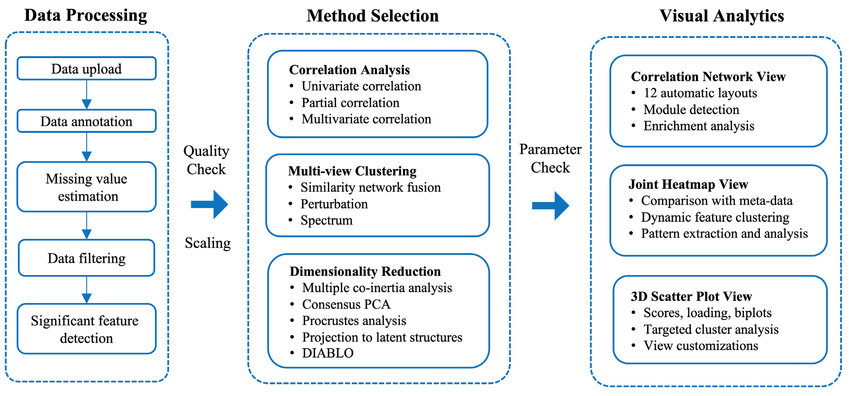
\includegraphics[scale=0.5]{images/workflow_omicsanalyst.png}
  \caption{Visión general del flujo de trabajo en OmicsAnalyst: (i) procesamiento de datos, (ii) selección de métodos de integración multivista, y (iii) análisis visual interconectado \cite{OmicsAnalyst}.}
  \label{fig:omicsanalyst_1}
\end{figure}

\newpage
La Figura~\ref{fig:omicsanalyst_1} ilustra un flujo típico de análisis multiómico incluyendo procesamiento de datos, selección de métodos (e.g., análisis de correlación, fusión de redes de similaridad, reducción de dimensionalidad como PCA/DIABLO) y visualización interactiva. OmicsAnalyst es una herramienta web ampliamente utilizada para este propósito, ofreciendo un entorno visual atractivo que facilita la integración y exploración de datos ómicos \cite{OmicsAnalyst}.\\


% ============ HACER TABLA =======================



% FLUJOS DE TRABAJO
\subsection{Flujos de trabajo multiómicos}
El análisis multiómico es un enfoque integral que combina datos provenientes de múltiples capas biológicas (genómica, transcriptómica, proteómica, metabolómica) para generar una visión holística de los sistemas biológicos. Este proceso sigue generalmente una arquitectura secuencial compuesta por etapas bien definidas, que aseguran la calidad, reproducibilidad y valor analítico de los resultados \cite{hasin2017multiomics_review} \cite{berger2021multiomics_pipeline}.

\begin{enumerate}
    % 1. Recolección y preprocesamiento de datos
    \item \textbf{Recolección y preprocesamiento de datos}
    Se inicia con la adquisición de datos ómicos desde múltiples fuentes (experimentos internos, consorcios, bases públicas), seguida de procesos de normalización, filtrado, control de calidad, estimación de valores faltantes y anotación contextual \cite{Krassowski_Das_Sahu_Misra_2025}. Cada tipo de ómica impone desafíos únicos (e.g., bajo conteo en transcriptómica, ruido técnico en metabolómica), por lo cual esta fase es crítica.

    % 2. Reducción de dimensionalidad
    \item \textbf{Reducción de dimensionalidad}
    Debido a la alta dimensionalidad típica de los datos ómicos, se aplican técnicas de reducción como \textit{Principal Component Analysis (PCA)}, \textit{t-distributed Stochastic Neighbor Embedding (t‑SNE)}, autoencoders o análisis de co-inercia múltiple. Esto permite visualizar los datos, detectar agrupamientos y mitigar la redundancia sin perder señal biológicamente relevante \cite{ramazzotti2022multiomics_dimensionality}.

    % 3. Integración de datos
    \item \textbf{Integración de datos}
    La integración puede estructurarse en tres estrategias principales:
    \begin{itemize}
        \item \textbf{Early integration:} combinación directa de las matrices, generando una única tabla combinada.
        \item \textbf{Intermediate integration:} algoritmos como \textit{MOFA}, \textit{SNF}, \textit{DIABLO} integran los datos manteniendo la identidad de cada capa y modelando relaciones latentes \cite{Argelaguet2018MOFA}.
        \item \textbf{Late integration:} cada capa se analiza por separado y los resultados se combinan en pasos posteriores.
    \end{itemize}

    % 4. Interpretación y visualización
    \item \textbf{Interpretación y visualización}
    Se exploran correlaciones, redes de interacción, firmas biológicas y relaciones funcionales utilizando herramientas como heatmaps, gráficos 3D, redes, árboles de decisión, y clústeres jerárquicos. Plataformas como \textit{OmicsAnalyst} permiten realizar estas visualizaciones de forma interactiva \cite{xia2022omicsanalyst}.

A continuación, se presenta un diagrama del pipeline en la plataforma \textit{OmicsAnalyst}, que agrupa el proceso en tres bloques principales: procesamiento de datos, selección de métodos e análisis visual interactivo (ver Figura~\ref{fig:omicsanalyst_2}):

\vspace{1em}
\begin{figure}[H]
    \centering
    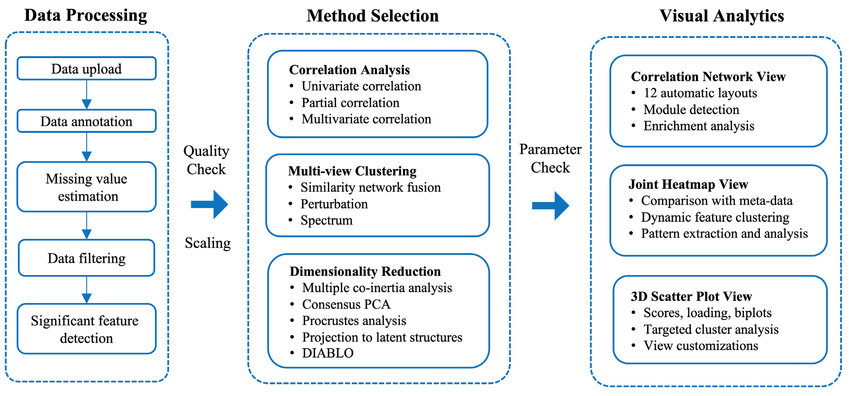
\includegraphics[width=0.9\textwidth]{images/workflow_omicsanalyst.png}
    \caption{Flujo general del análisis multiómico en OmicsAnalyst, dividido en procesamiento, selección de método y análisis visual.}
    \label{fig:omicsanalyst_2}
\end{figure}

    % 5. Ejemplos de frameworks multiómicos
    \item \textbf{Ejemplos de frameworks multiómicos}
    El uso de frameworks específicos permite automatizar y reproducir estos flujos. Por ejemplo:
    
    \begin{itemize}
      \item \textbf{MiBiOmics}: integración basada en co-inercia y redes (PCA, WGCNA) \cite{gautier2021mibiomics}.
      \item \textbf{Omix}: contiene contenedores modulares para cada etapa y modelos como \textit{MOFA+} y \textit{DIABLO}.
      \item \textbf{Holomics}: integración supervisada multietapa con enfoque modular.
    \end{itemize}
    
    \vspace{1em}
    \begin{figure}[H]
        \centering
        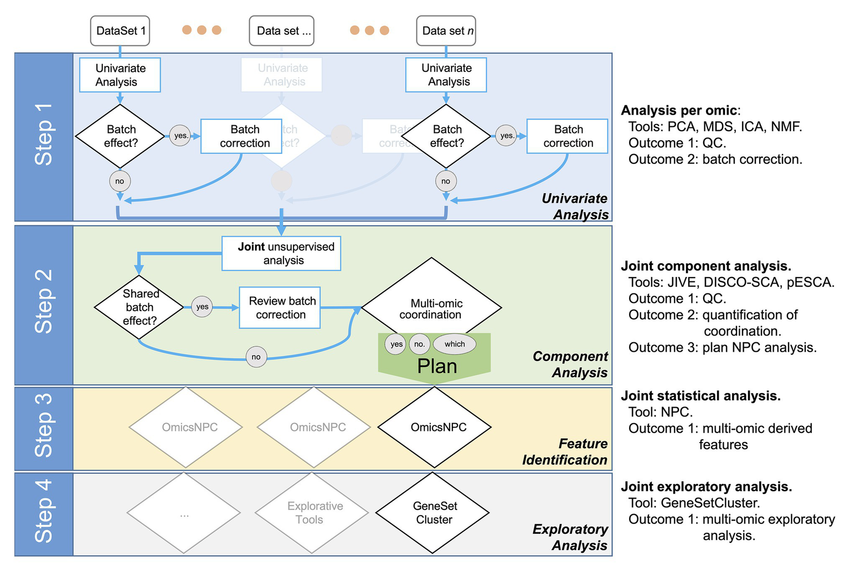
\includegraphics[width=0.95\textwidth]{images/Workflow-diagram-of-the-multi-omics-analysis-framework.png}
        \caption{Ejemplo de flujo de trabajo multiómico para análisis integrativo con pasos desde la carga hasta la fusión de datos.}
        \label{fig:workflow_framework}
    \end{figure}

    % 6. Entornos reproducibles y orquestación
    \item \textbf{Entornos reproducibles y orquestación}
    La implementación de herramientas como Nextflow y Airflow permite definir flujos de trabajo declarativos, modulares y reproducibles, integrando contenedores como Docker o Singularity junto con control de versiones. Esta capacidad resulta crítica en escenarios multiómicos, donde se manipulan datos heterogéneos, de alta dimensionalidad y alta variabilidad técnica \cite{di_tommaso2017nextflow} \cite{ewels2020nfcore} \cite{yasmin2024empirical}.\\

    Más allá de su función operativa, estos sistemas de orquestación representan una arquitectura conceptual robusta capaz de transformar datos complejos en estructuras analíticas coherentes, trazables y reutilizables. Como lo demuestra el estudio empírico \cite{yasmin2024empirical}, los principales desafíos en Airflow—la definición y ejecución de DAGs y la configuración del entorno distribuido—resaltan la necesidad de este enfoque integrado. Así, se establece una base sólida para análisis avanzados con modelos de aprendizaje automático, descubrimiento de biomarcadores, visualización integrada y toma de decisiones científicamente informada.


\end{enumerate}











% \begin{enumerate}
%   \item \textbf{Recolección y preprocesamiento de datos}: incluye la obtención de datos desde diversas ómicas (genómica, transcriptómica, proteómica, metabolómica), seguidos de limpieza, normalización, filtrado de valores faltantes y control de calidad de cada capa de datos \cite{Lehmann2020multiomics_metabolomics_review} \cite{Krassowski2020multiomics_review}.

%   \item \textbf{Reducción de dimensionalidad}: es la aplicación de técnicas como \emph{PCA}, \emph{t‑SNE}, autoencoders o análisis de componentes latentes para reducir el número de variables sin perder información relevante \cite{Tomazou2021multiomics_covid}.

%   \item \textbf{Integración de datos:}  
%     Estrategias según el momento de fusión:
%     \begin{itemize}
%       \item \emph{Early integration}: concatenación directa de las matrices ómicas.
%       \item \emph{Intermediate integration}: métodos conjuntos como MOFA o Similarity Network Fusion (SNF) para capturar factores latentes sin concatenar directamente las matrices \cite{Lehmann2020multiomics_metabolomics_review}.
%       \item \emph{Late integration}: análisis independientes por capa, combinando resultados en etapas finales.
%     \end{itemize}

%     \item \textbf{Interpretación biológica y visualización}: Identificación de biomarcadores y patrones biológicos a través de análisis estadísticos, redes de correlación y visualizaciones interactivas (heatmaps, gráficos 3D), facilitadas por plataformas como OmicsAnalyst \cite{OmicsAnalyst}\cite{Planell2021stategra}.
% \end{enumerate}

% Un resumen visual de este pipeline se muestra en la Figura~\ref{fig:omicsanalyst_2}, tomada de OmicsAnalyst, que divide el proceso en tres fases clave: procesamiento de datos, selección de métodos y análisis visual interactivo:

% \begin{figure}[h!]
%     \centering
%     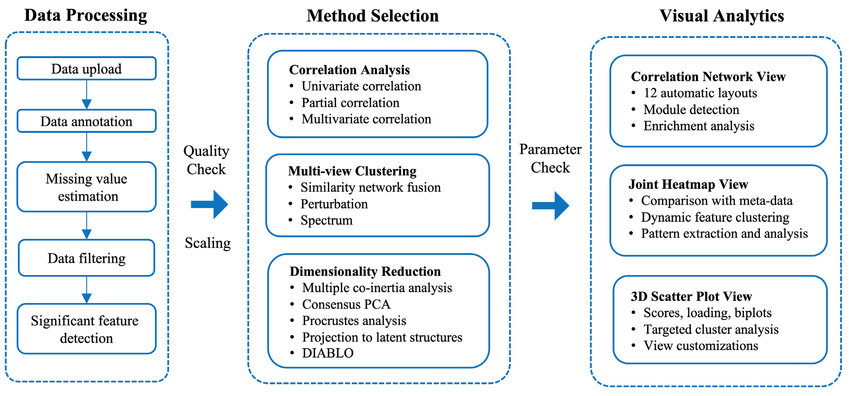
\includegraphics[width=0.8\textwidth]{images/workflow_omicsanalyst}
%     \caption{Flujo general del pipeline multiómico en la plataforma OmicsAnalyst: procesamiento, integración y visualización interactiva.}
%     \label{fig:omicsanalyst_2}
% \end{figure}

% \medskip

% \textbf{Ejemplos de herramientas y frameworks}:  
% Plataformas como \textit{Holomics} integran workflows tipo Holomics: carga de datos, análisis uniómico inicial y análisis multiómico supervisado (DIABLO o similares) en tres etapas principales \cite{turn0search3}. Aplicaciones como MiBiOmics permiten ejecutar preprocesamiento, análisis exploratorio (PCA, WGCNA), y finalmente integración multiómica basada en co-inercia o redes \cite{turn0search0}. Herramientas como Omix estructuran el pipeline en contenedores multimodales, procesamiento, análisis por ómica y fusión vertical con modelos como MOFA o DIABLO, seguidos de análisis funcionales downstream \cite{turn0search2}.


% \medskip

% \textbf{Importancia de orquestadores y entornos reproducibles}:  
% Sistemas como \textit{Nextflow} o \textit{nf‑core} permiten construir pipelines reproducibles y escalables, portables a diferentes infraestructuras computacionales, cuidando versiones, contenedores y trazabilidad técnica \cite{turn0search14} \cite{turn0search6}. Esto es especialmente útil en análisis complejos con múltiples muestras y tecnologías ómicas.

% \medskip

% Este pipeline no es solo una secuencia técnica, sino una arquitectura conceptual que permite transformar datos heterogéneos y de alta dimensionalidad en conocimiento integrable y visualizable. Así, se establece una base sólida para respaldar análisis posteriores de IA, descubrimiento de biomarcadores y toma de decisiones fundamentadas en datos.


% % Origen y aplicaciones de datos multiómicos
% \subsection{Origen y aplicaciones de datos multiómicos}
% Las fuentes de datos incluyen muestras clínicas, modelos celulares/animales, y repositorios públicos como MetaboLights \cite{yurekten2024metabolights}.

% \subsection{Principios FAIR y calidad de datos}
% Los datos multiómicos deben cumplir con los principios FAIR estableciendo identificadores únicos, APIs estándar, vocabularios controlados y metadatos ricos \cite{wilkinson2016fair_principles}. Esto exige:

% \begin{itemize}
%   \item Identificadores únicos (p.ej. DOI, UUID).
%   \item APIs REST o FTP para interoperabilidad.
%   \item Ontologías estandarizadas y metadatos enriquecidos.
%   \item Licencias y datos lisibles por máquina \cite{wilkinson2016fair_principles}.
% \end{itemize}

% \subsection{IA explicable (XAI) en entornos multiómicos}
% Técnicas como SHAP y LIME permiten entender las predicciones de modelos complejos, otorgando transparencia y respaldo científico en aplicaciones biomédicas \cite{salih2023perspective_shap_lime}.

% \subsection{Gestión documental integrada}
% Para documentar flujos de datos multiómicos es esencial un repositorio compatible FAIR, combinado con ELN/LIMS, contenedores y orquestación de pipelines mediante Airflow o Nextflow.



\newpage
\section{Bases de Datos}
\input{Marco Teórico/Bases de datos}
\newpage
\section{Protocolos de Comunicación Industriales}
% El avance de las tecnologías de la información ha permitido el desarrollo de sofisticadas herramientas de visualización y análisis de datos, fundamentales para la toma de decisiones en entornos empresariales dinámicos. En el contexto de la CVC y la sostenibilidad, estas herramientas facilitan la interpretación de grandes volúmenes de datos y el monitoreo en tiempo real de indicadores estratégicos, siendo factotes cruciales para que las Pymes puedan competir en mercados cada vez más digitales. Entre las principales herramientas utilizadas se destacan:


% \begin{itemize}
%     \item \textbf{Plataformas de Dashboards Interactivos:}  
%     \emph{Power BI} y \emph{Tableau} son dos de las plataformas líderes en la creación de tableros interactivos. Estas herramientas permiten integrar datos provenientes de múltiples fuentes, aplicar filtros dinámicos y presentar la información de manera gráfica, facilitando la identificación de tendencias y patrones relevantes. Microsoft, por ejemplo, ha destacado en su noticia “Microsoft dota de inteligencia de datos a las empresas pequeñas con Power BI” cómo esta plataforma democratiza el acceso a análisis avanzados, permitiendo a las Pymes transformar grandes volúmenes de datos en información estratégica para la toma de decisiones \cite{PowerBI_News2023}.
    
%     \item \textbf{Librerías de Visualización en Python:}  
%     Herramientas como \emph{Plotly}, \emph{Dash} y \emph{Seaborn} ofrecen una gran flexibilidad para desarrollar soluciones personalizadas de visualización. Estas librerías permiten crear gráficos interactivos, heatmaps y dashboards que se integran en aplicaciones web, facilitando el acceso a la información en tiempo real y adaptándose a las necesidades específicas de los modelos predictivos.
    
%     \item \textbf{Sistemas de Integración y Consolidación de Datos:}  
%     La efectividad de las herramientas de visualización depende en gran medida de la capacidad para integrar y consolidar datos de diversas fuentes. Herramientas ETL (Extract, Transform, Load) y bases de datos de alto rendimiento permiten centralizar la información, garantizando que los datos presentados sean consistentes y actualizados.
% \end{itemize}

% El uso combinado de estas tecnologías no solo permite visualizar el output de los modelos predictivos, sino que también posibilita la generación de informes personalizados y el monitoreo de indicadores clave (KPIs) relacionados con la CVC y la sostenibilidad. La Figura~\ref{fig:Dashboard_Ejemplo} muestra un ejemplo de un tablero interactivo desarrollado en Power BI por Microsoft para monitorear estos indicadores en tiempo real, facilitando la toma de decisiones estratégicas en Pymes \cite{PowerBI_News2023}.

% \begin{figure}[h!]
%   \centering
%   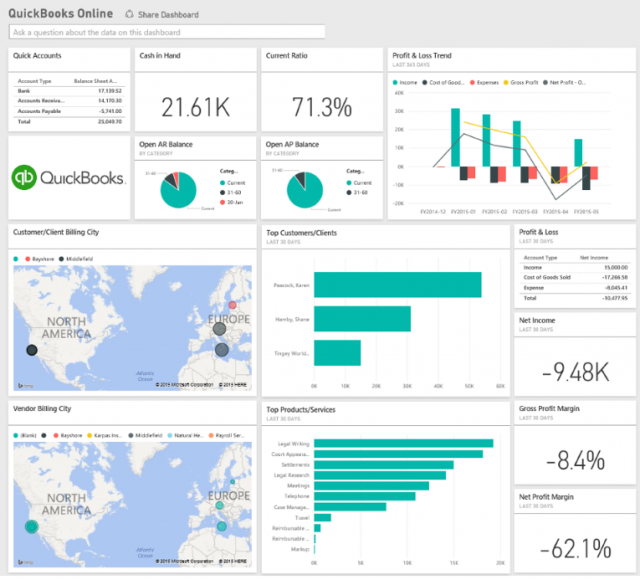
\includegraphics[width=0.75\textwidth]{images/Power-BI_QBO_Pymespng.png}
%   \caption{Ejemplo de tablero interactivo para la visualización de indicadores estratégicos en Pymes.}
%   \label{fig:Dashboard_Ejemplo}
% \end{figure}







% % % ====================== OPC UA ======================
% % Los protocolos de comunicación forman parte de nuestra investigación, para el entendimiento de las comunicaciones que se presentan en la funcionalidad de la celda de Manufactura Flexible del CAP. Esto con el fin de conocer su funcionamiento a profundidad y de los protocolos y normas existentes detrás de estas comunicaciones.\newline

% % \subsection{OPC UA (Arquitectura Unificada de Comunicaciones de Plataforma
% % Abierta)}
% % Es una arquitectura orientada a servicios independiente de la plataforma que integra toda la funcionalidad de las especificaciones individuales de OPC Classic en un marco extensible que proporciona soluciones más robustas, seguras y escalables para la comunicación industrial \cite{OPC_Foundation_2019_UA} \cite{OPC_Foundation_2020_Classic}. \\

% % A diferencia de OPC Classic, OPC UA puede funcionar en diferentes sistemas operativos, como Windows, Linux y otros. Utiliza protocolos estándar de Internet, como TCP/IP y HTTPS, para la comunicación, lo que facilita la interoperabilidad entre dispositivos y aplicaciones en entornos heterogéneos. Una de las principales ventajas de OPC UA es su enfoque en la seguridad. Proporciona mecanismos de autenticación, autorización y cifrado de extremo a extremo para proteger la comunicación y los datos transmitidos. Además, ofrece características avanzadas, como un modelo de información flexible, soporte para datos históricos, notificación de eventos y gestión de alarmas \cite{OPC_Foundation_2019_UA} \cite{paessler} \cite{siemens_ag_2017}. \\

% % OPC-UA se ha convertido en el estándar de facto para la comunicación industrial y ha sido adoptado por muchas empresas y organizaciones en todo el mundo. La norma \textbf{IEC 62541} define las especificaciones técnicas para la implementación de OPC UA, brindando un marco común y coherente para su implementación y uso en diversos sectores de la industria \cite{Person_ICONICS_INC_2008} \cite{INTERNATIONAL_ELECTROTECHNICAL_COMMISSION_2020}.\\

% % Las principales especificaciones técnicas definidas por la norma \textbf{IEC 62541} son las siguientes:

% % \begin{enumerate}
% %   \item \textbf{Modelo de información:} Se establecen las estructuras de datos y la semántica utilizada para describir la información intercambiada entre los sistemas a través de OPC UA. Esto incluye la definición de nodos, atributos, métodos y eventos.
% %   \item \textbf{Protocolo de comunicación:} Se especifica el protocolo de comunicación utilizado para la transferencia de datos entre los sistemas. OPC UA utiliza un modelo cliente-servidor, donde los clientes solicitan y reciben datos de los servidores. El protocolo puede basarse en TCP/IP y soportar diferentes mecanismos de transporte y seguridad.
% %   \item \textbf{Seguridad:} Se definen los mecanismos de seguridad utilizados para proteger la comunicación y los datos transmitidos en OPC UA. Esto incluye autenticación, autorización, cifrado y firma digital, entre otros aspectos.
% %   \item \textbf{Descubrimiento y conexión:} Se describe cómo los clientes pueden descubrir y conectarse a los servidores OPC UA disponibles en la red. Esto puede implicar la resolución de nombres, la búsqueda de servicios de directorio y la negociación de las opciones de comunicación.
% %   \item \textbf{Historial de datos:} Se establece cómo se almacenan y acceden a los datos históricos en OPC UA. Esto puede incluir la capacidad de almacenamiento local en los servidores y la consulta de datos históricos por parte de los clientes.
% %   \item \textbf{Alarmas y eventos:} Se establece el mecanismo para el manejo de alarmas y eventos en OPC UA. Permite a los servidores notificar a los clientes sobre cambios de estado, condiciones de error o eventos relevantes.

% % \end{enumerate}

% % % ====================== Ethernet % ======================
% % \subsection{Ethernet Industrial}
% % Es el uso de Ethernet en un entorno industrial con protocolos que proporcionan determinismo y control en tiempo real. Los protocolos para Ethernet industrial incluyen EtherCAT , EtherNet/IP , PROFINET , POWERLINK , SERCOS III , CC-Link IE y Modbus TCP \cite{Lin_Pearson_TexasInst_2018}. En el caso de la celda de manufactura del CAP, esta utiliza el protocolo de Modbus TCP (también Modbus TCP/IP), el cual es una extensión de Modbus RTU con una interfaz TCP que se ejecuta en Ethernet a través del puerto 502 y fue desarrollado originalmente por Schneider Electric. Además, Modbus es un bus serial sencillo, robusto y libre de derechos de autor que es fácil de implementar y funciona en enlaces físicos RS-232 o RS-485 con velocidades de hasta 115K baudios. \cite{ACROMAG_INCORPORATED_2005} \cite{ENCODER_PRODUCTS_COMPANY_2019}.\\

% % Por otro lado, Ethernet se está convirtiendo en omnipresente y rentable, con enlaces físicos comunes y mayor velocidad, por ello, muchos protocolos de comunicación industrial se están pasando a soluciones basadas en esta tecnología, permitiendo así una topología de red flexible y un número de nodos en el sistema \cite{Lin_Pearson_TexasInst_2018}.

% % % ====================== TCP/IP % ======================
% % \subsection{Modbus TCP/IP }
% % Fue desarrollado bajo la unión del protocolo de aplicación Modbus con la transmisión Ethernet \textbf{IEEE 802.3} tradicional. El Protocolo de control de transporte (TCP) reside una capa por encima del Protocolo de Internet (IP) y es responsable de transportar los datos de la aplicación y hacerlos seguros, mientras que IP es responsable del direccionamiento real y la entrega de los datos \cite{Andersdotter_Lansford_Law_Marks_Myles_2023}. \\

% % Por un lado, el paquete TCP se inserta en la porción de datos del paquete IP debajo de él, mientras que IP en sí mismo es un protocolo no seguro y sin conexión y debe funcionar junto con el TCP superpuesto para poder operar. De esta forma, TCP generalmente se considera la capa superior de la plataforma IP que sirve para garantizar la transferencia segura de datos \cite{ACROMAG_INCORPORATED_2005}. Para implementar una comunicación Modbus se deben tener en cuenta las siguientes reglas según la organización de Modbus \cite{Modbus_Organization_2006}:

% % \begin{enumerate}
% %     \item Sin requisitos explícitos del usuario, se recomienda implementar la gestión automática de conexiones TCP.
% %     \item Se recomienda mantener la conexión TCP abierta con un dispositivo remoto y no abrirla y cerrarla para cada transacción MODBUS/TCP. Observación: Sin embargo, el cliente MODBUS debe ser capaz de aceptar una solicitud de cierre del servidor y cerrar la conexión. . La conexión se puede reabrir cuando sea necesario.
% %     \item Se recomienda que un Cliente MODBUS abra un mínimo de conexiones TCP con un servidor MODBUS remoto (con la misma dirección IP). Una conexión por aplicación podría ser una buena opción.
% %     \item Se pueden activar varias transacciones MODBUS simultáneamente en la misma conexión TCP. Observación: si se hace esto, entonces se debe usar el identificador de transacción MODBUS para identificar de manera única las solicitudes y respuestas coincidentes.
% %     \item En el caso de una comunicación bidireccional entre dos entidades MODBUS remotas (cada una de ellas es cliente y servidor), es necesario abrir conexiones separadas para el flujo de datos del cliente y para el flujo de datos del servidor.
% %     \item Una trama/frame TCP debe transportar solo una ADU MODBUS. Se desaconseja enviar múltiples solicitudes o respuestas MODBUS en la misma PDU TCP.
% % \end{enumerate}

% % % ====================== Comunicación Serial RS232 y señales digitales I/O ======================
% % \subsection{Comunicación Serial RS232 y señales digitales I/O }
% % El protocolo de comunicación RS232 (Estándar Recomendado 232 por sus siglas en inglés) fue introducido por primera vez en 1960 por la Electronic Industries Association (EIA)   es uno de los más antiguos pero populares que se utiliza a nivel industrial. Este es un tipo de tipo de comunicación serial utilizada para la transmisión de datos normalmente en distancias medias \cite{Sharma_2018}. No obstante, el estándar ha cambiado de nombre varias veces durante su historia a medida que la organización cambió su nombre, y ha sido conocido como EIA RS-232, EIA 232 y, más recientemente, como TIA 232 desde 1988 por la Telecommunications Industry Association (TIA). \\

% % Debido a que RS-232 se usa más allá del propósito original de interconectar un terminal con un módem, se han desarrollado estándares sucesores para abordar las limitaciones. Los problemas con el estándar RS-232 incluyen \cite{Horowitz_Hill_1989}:

% % \begin{itemize}
% %     \item Las grandes oscilaciones de voltaje y el requisito de suministros positivos y negativos aumentan el consumo de energía de la interfaz y complican el diseño de la fuente de alimentación. El requisito de oscilación de voltaje también limita la velocidad superior de una interfaz compatible.
% %     \item La señalización de un solo extremo referida a una tierra de señal común limita la inmunidad al ruido y la distancia de transmisión.
% %     \item La conexión multipunto entre más de dos dispositivos no está definida. Si bien se han ideado "soluciones alternativas" multipunto, tienen limitaciones en cuanto a velocidad y compatibilidad.
% %     \item El estándar no aborda la posibilidad de conectar un DTE directamente a un DTE, o un DCE a un DCE. Se pueden usar cables de módem nulo para lograr estas conexiones, pero estos no están definidos por el estándar, y algunos de estos cables usan conexiones diferentes que otros.
% %     \item No se especifica ningún método para enviar energía a un dispositivo. Si bien se puede extraer una pequeña cantidad de corriente de las líneas DTR y RTS, esto solo es adecuado para dispositivos de bajo consumo, como ratones .
% %     \item El conector D-sub de 25 pines recomendado en el estándar es grande en comparación con la práctica actual.
% % \end{itemize}

% % En cuanto a las máquinas de la celda de manufactura del CAP, los controladores de dispositivo tanto para los tornos como para las fresadoras Denford se comunican con las herramientas de máquina de dos maneras diferentes: Enlaces seriales RS232 y señales digitales de Entrada y Salida (I/O) \cite{DenfordLTD_2002}.\\

% % En el caso de RS232 se utiliza para la descarga de programas: control numérico directo (DNC) y verificación detallada del estado. Se debe conectar un cable de RS232 desde un puerto serial en la PC de la celda supervisora al puerto serial externo en la máquina herramienta. Para comunicarse a través del enlace serial, tanto la máquina herramienta como el controlador del dispositivo deben usar la misma configuración \cite{DenfordLTD_2002}. \\

% % Las señales I/O se conectan directamente desde el módulo de interfaz al puerto de entrada y salida auxiliar de la máquina. Hay dos líneas de entrada y dos líneas de salida que se pueden usar para transmitir información de estado de bajo nivel al controlador del dispositivo. Todas las herramientas Denford están conectadas al módulo de interfaz de I/O en los puertos 2A o 2B \cite{DenfordLTD_2002}. El puerto auxiliar proporciona dos entradas a la herramienta, dos salidas de la máquina y un circuito de parada de emergencia. Las entradas y salidas hacia y desde la herramienta corresponden a cuatro códigos 'M':

% % \begin{itemize}
% %     \item M62: salida 1 activada.
% %     \item M63: salida 2 activada.
% %     \item M64: salida 1 desactivada
% %     \item M65: salida 2 desactivada
% % \end{itemize}



\newpage
\section{Estado del Arte}
% Para la realización de este trabajo se consultaron diferentes investigaciones enfocadas en el análisis de sostenibilidad y creación de valor compartido en pequeñas y medianas empresas, mediante el uso de modelos predictivos y enfoques multivariantes. Estos trabajos se resumen a continuación:

% % ----------------------------------------------------------------------------------------
% \subsection{Using structural equation modeling to test environmental performance in small and medium-sized manufacturers: can SEM help SMEs?}
% En este artículo, los autores exploran la utilidad del modelado de ecuaciones estructurales (SEM) como metodología para validar un modelo de desempeño ambiental dirigido a pequeñas y medianas empresas manufactureras (PYMEs), particularmente en los sectores de plásticos y metales fabricados. El modelo propuesto se fundamenta en los Criterios Baldrige de Excelencia, adaptados para enfocar la gestión ambiental dentro de las PYMEs.\\

% El estudio se basó en una muestra de 458 empresas, empleó el Modelado de Ecuaciones Estructurales (SEM) mediante la herramienta LISREL para examinar las interconexiones entre variables latentes clave: liderazgo, planificación, recursos humanos, gestión ambiental, análisis de información y resultados ambientales. Si bien el modelo global presentó un ajuste razonable, algunas relaciones con los resultados ambientales no fueron estadísticamente significativas, lo que sugiere que las PYMEs enfrentan dificultades para comprender y medir eficazmente este concepto. Además, se enfatiza la urgencia de refinar la definición de los resultados ambientales y de adaptar las herramientas y modelos preexistentes, diseñados principalmente para grandes corporaciones, a las condiciones operativas específicas de las PYMEs \cite{hussey2007using}.


% % ----------------------------------------------------------------------------------------
% \subsection{Using structural equation modeling to test environmental performance
% in small and medium-sized manufacturers: can SEM help SMEs}
% En este artículo se analiza la aplicación del modelado de ecuaciones estructurales (SEM) para la validación de modelos de desempeño ambiental en pequeñas y medianas empresas (PYMEs). Los autores describen cómo la utilización de SEM permite establecer relaciones causales entre variables latentes que representan componentes esenciales en la gestión ambiental, tales como el liderazgo, la planificación, la implicación de recursos humanos y la implementación de prácticas de gestión ambiental.\\

% El estudio, basado en la adaptación de criterios internacionales (como los Criterios Baldrige) al contexto de las PYMEs, demuestra que la metodología proporciona un ajuste razonable del modelo global. Sin embargo, se destaca la necesidad de precisar la definición de “resultados ambientales”, ya que algunos caminos del modelo no resultaron estadísticamente significativos. Este trabajo es relevante para el presente estudio, ya que respalda la viabilidad de enfoques multivariantes para integrar aspectos de sostenibilidad ambiental y creación de valor compartido en las PYMEs \cite{hussey2007ecuaciones}.\\

% Estos hallazgos son pertinentes para nuestro trabado, dado que analiza el contexto de las Pymes implementando SEM y la relación entre variables latentes, ofreciendo resultados técnicos sobre la pertinencia de algunas variables. Dichos hallazgos resultan importantes como insumo para identificar y descartar variables del modelo de estimación.

% % ----------------------------------------------------------------------------------------
% \subsection{The impact of creating shared value strategy on corporate sustainable development: From resources perspective}
% En este artículo, Li et al. (2023) examinan el impacto de la estrategia de creación de valor compartido en el desarrollo sostenible corporativo, desde una perspectiva centrada en los recursos. El estudio se enfoca en cómo la integración y gestión de recursos en pequeñas y medianas empresas (PYMEs) puede potenciar tanto la competitividad como la sostenibilidad ambiental y social. A través de un análisis empírico y el uso de modelos multivariantes, los autores identifican factores críticos que facilitan la implementación exitosa de estrategias de valor compartido, destacando la importancia de alinear los objetivos económicos con los ambientales. Este enfoque permite a las PYMEs generar ventajas competitivas sostenibles, mejorando su desempeño global y promoviendo prácticas que contribuyen al desarrollo sostenible. La investigación aporta un marco conceptual y metodológico relevante para el presente trabajo, ya que respalda la integración de modelos multivariantes para predecir la creación de valor compartido y su relación con la sostenibilidad ambiental en el contexto de las PYMEs \cite{li2023impact}.

% % ----------------------------------------------------------------------------------------
% \subsection{Strategic Sense-Making and Value Creation in SMEs}
% En este artículo se explora el rol del sense-making estratégico en la creación de valor en las PYMEs. Los autores analizan cómo los procesos cognitivos y la interpretación de la información por parte de los directivos permiten identificar y aprovechar oportunidades para generar valor compartido. En este sentido, el estudio destaca que la capacidad de sentido estratégico facilita la alineación de los recursos internos con las demandas del entorno, lo que resulta fundamental para impulsar innovaciones y mejorar la competitividad. Mediante un enfoque empírico, se examinan casos y se aplican métodos cuantitativos para evidenciar que un adecuado proceso de sense-making contribuye a fortalecer la capacidad de las PYMEs para generar valor tanto interno como en su relación con el mercado. Estos hallazgos son relevantes para el presente trabajo, ya que aportan elementos teóricos y prácticos que pueden integrarse en modelos multivariantes orientados a predecir la creación de valor compartido y su impacto en la sostenibilidad ambiental \cite{SenseMakingValueCreation}.

% % ----------------------------------------------------------------------------------------
% \subsection{Determinants of Environmental, Financial, and Social Sustainability}
% En este artículo se analizan de manera integral los determinantes que influyen en la sostenibilidad en tres dimensiones fundamentales: ambiental, financiera y social. Los autores adoptan un enfoque multivariante para identificar cómo factores internos —como la disponibilidad y la gestión de recursos, las capacidades organizacionales y las prácticas de innovación—, junto con elementos externos del entorno competitivo y regulatorio, inciden en el desempeño sostenible de las organizaciones.\\

% \noindent El estudio proporciona evidencia empírica de que la alineación estratégica y la integración de políticas de sostenibilidad en el modelo de negocio son cruciales para mejorar el desempeño en las tres áreas analizadas. Aunque la investigación no se centra exclusivamente en PYMEs, los hallazgos ofrecen importantes lecciones sobre cómo las pequeñas y medianas empresas pueden optimizar la creación de valor compartido mediante la adopción de estrategias que combinen la eficiencia ambiental con resultados financieros y beneficios sociales. Esto respalda la premisa del presente trabajo, que propone el desarrollo de modelos multivariantes para predecir la creación de valor compartido y su relación con la sostenibilidad ambiental en PYMEs \cite{DeterminantsSustainability}.




%%%%%%% CONCEBIR %%%%%%%%%%%%%
\chapter{Definición de Requisitos}
\section{Descripción del Caso de Estudio}
% \section{Variables determinantes de la CVC en Pymes}
% Para alcanzar este objetivo se realizará un análisis bibliométrico con el propósito de identificar y justificar teóricamente las principales variables de la CVC. Adicionalmente, este análisis permitirá profundizar en este campo a partir del estudio de los desarrollos recientes, las posibles áreas de aplicación y la importancia de la CVC en las Pymes de países en desarrollo. En ese sentido, se espera explorar los aspectos emergentes, las tendencias actuales y realizar el metanálisis mediante la realización de una revisión sistemática de la literatura disponible sobre CVC en las Pymes publicados en revistas revisadas por pares durante el período 2000-2024.
\newpage
\section{Especificación de Requisitos}
% Al analizar las características y necesidades de las Pymes en Barranquilla, se han establecido los siguientes requisitos para el diseño de un sistema que facilite la implementación efectiva de la Creación de Valor Compartido:

% \begin{enumerate}
%     \item \textbf{Adaptabilidad y Escalabilidad del Sistema}
%     \begin{enumerate}
%         \item El sistema debe ser adaptable a diferentes sectores y tamaños de Pymes, permitiendo su escalabilidad y personalización según las necesidades específicas de cada empresa.
%         \item Debe permitir la integración con herramientas existentes y futuras, facilitando la evolución tecnológica y organizacional de las Pymes.
%     \end{enumerate}
    
%     \item \textbf{Gestión de Datos para la Sostenibilidad}
%     \begin{enumerate}
%         \item El sistema debe contar con una base de datos robusta que permita el almacenamiento y análisis de indicadores clave relacionados con la sostenibilidad ambiental, social y económica.
%         \item Debe facilitar la recopilación de datos sobre consumo de recursos, emisiones, gestión de residuos y otros aspectos ambientales relevantes.
%     \end{enumerate}
    
%     \item \textbf{Interfaz de Usuario Intuitiva}
%     \begin{enumerate}
%         \item El sistema debe ofrecer una interfaz de usuario amigable que permita a los empleados de las Pymes ingresar y consultar información de manera eficiente.
%         \item Debe incluir módulos específicos para la gestión de proyectos de CVC, seguimiento de indicadores de sostenibilidad y generación de informes.
%     \end{enumerate}
    
%     \item \textbf{Soporte para la Toma de Decisiones Estratégicas}
%     \begin{enumerate}
%         \item El sistema debe proporcionar herramientas analíticas que faciliten la identificación de oportunidades para la creación de valor compartido y la mejora continua en sostenibilidad.
%         \item Debe permitir la simulación de escenarios y el análisis de impacto de diferentes estrategias empresariales en términos de sostenibilidad.
%     \end{enumerate}
    
%     \item \textbf{Cumplimiento Normativo y Reporte de Información}
%     \begin{enumerate}
%         \item El sistema debe estar alineado con las normativas locales e internacionales relacionadas con la sostenibilidad y la responsabilidad social empresarial.
%         \item Debe facilitar la generación de informes requeridos por entidades regulatorias y partes interesadas, asegurando la transparencia y rendición de cuentas.
%     \end{enumerate}
    
%     \item \textbf{Capacitación y Soporte Técnico}
%     \begin{enumerate}
%         \item El sistema debe incluir recursos de capacitación para los usuarios, promoviendo una cultura organizacional orientada a la sostenibilidad y la innovación.
%         \item Debe contar con soporte técnico accesible para resolver problemas y garantizar el funcionamiento continuo del sistema.
%     \end{enumerate}
% \end{enumerate}

%%%%%%% DISEÑAR %%%%%%%%%%%%%
\chapter{Diseño del Sistema de Información}

% Este capítulo representa un punto clave en el desarrollo del trabajo de grado, al centrarse en el cumplimiento del segundo objetivo específico: \textbf{desarrollar un modelo multivariante que permita explicar la relación entre la creación de valor compartido (CVC) y la sostenibilidad ambiental en PYMEs}. Para ello, se adopta una estrategia metodológica rigurosa y adecuada al tipo de datos y naturaleza del fenómeno investigado, haciendo uso de técnicas avanzadas de análisis estructural. 

% \textbf{
% \section{Técnicas aplicadas }
% }


% El enfoque metodológico elegido fue el \textbf{Modelado de Ecuaciones Estructurales (SEM)}, el cual es especialmente potente para estudiar \textbf{relaciones complejas entre variables latentes}, permitiendo validar modelos teóricos y establecer relaciones de causalidad a partir de datos observados. El proceso se divide en dos fases principales:

% \textbf{
% \subsection{Fase 1: Análisis Factorial Confirmatorio (AFC) }
% }

% En esta fase se parte de los constructos teóricos identificados previamente mediante el \textbf{Análisis Factorial Exploratorio (AFE)} desarrollado en el capítulo anterior, los cuales agrupan 18 variables en \textbf{tres dimensiones fundamentales}:

% \begin{itemize}
%     \item \textbf{Dimensión interna}: cultura organizacional, liderazgo, gestión del conocimiento.
%     \item \textbf{Dimensión externa}: relación con stakeholders, alianzas, impacto social.
%     \item \textbf{Dimensión ambiental}: eficiencia en el uso de recursos, políticas sostenibles, gestión de residuos.
% \end{itemize}
% El AFC permite \textbf{confirmar la validez estructural} de estas dimensiones, asegurando que los ítems observados (preguntas de la encuesta) efectivamente representan los constructos teóricos esperados. Se evalúan así:

% \begin{itemize}
%     \item \textbf{Cargas factoriales}: deben superar el umbral de 0.5 para considerar que un ítem se asocia adecuadamente a un factor.
%     \item \textbf{Validez convergente}: que los ítems de un mismo constructo se correlacionan fuertemente.
%     \item \textbf{Validez discriminante}: que los constructos se diferencian adecuadamente entre sí.


% \textbf{
% \subsection{Fase 2: Modelado estructural }
% }

% Una vez validados los constructos, se procede al desarrollo del modelo estructural, el cual especifica las \textbf{relaciones de influencia entre las variables latentes}.

% \begin{itemize}
%     \item Se establecen \textbf{relaciones causales directas} entre las dimensiones de gestión interna y externa, y la variable dependiente: el nivel de sostenibilidad ambiental.
%     \item Se estiman \textbf{coeficientes estandarizados ($\beta$)} que indican la \textbf{intensidad y dirección de las relaciones}.
%     \item Por ejemplo, un valor positivo y significativo de β entre “liderazgo” y “sostenibilidad ambiental” sugiere que a mayor liderazgo, mayor sostenibilidad ambiental percibida.
% \end{itemize}


% \textbf{ Validación del modelo }

% El modelo estructural se valida mediante \textbf{índices de ajuste global}, ampliamente aceptados en la literatura científica:

% \begin{itemize}
%     \item \textbf{CFI (Comparative Fit Index)}: compara el modelo propuesto con un modelo nulo. Se exige un valor > 0.90 para considerar buen ajuste.
%     \item \textbf{TLI (Tucker-Lewis Index)}: penaliza por complejidad, también debe ser > 0.90.
%     \item \textbf{RMSEA (Root Mean Square Error of Approximation)}: mide el error por grado de libertad. Debe ser < 0.08 para indicar un ajuste aceptable.
%     \item Otros índices como el \textbf{Chi-cuadrado / df}, \textbf{SRMR}, o el \textbf{AIC} pueden haberse considerado, aunque no se detallan explícitamente.
% \end{itemize}
% La validez estadística del modelo da paso a la interpretación sustantiva de los resultados.

% \end{itemize}
\section{Base de Datos}
% \subsection{Diseño conceptual}
% Como se mencionó en la introducción del proyecto, el desarrollo de la base de datos se realizará a partir del lenguaje Cypher y de la plataforma de desarrollo Neo4j. Para el primer diseño, se pensó en la representación de máquinas y elementos existentes de la celda, como un nodo en la base de datos. Es decir, la celda cuenta con estaciones, sus estaciones con máquinas, las máquinas fabrican piezas y estas piezas necesitan de material disponible.\\

% Estas relaciones, son las que decidimos optar como las etiquetas que permitieran conectar a los nodos. Por tal razón, el primer diseño de la celda se presenta en la figura \ref{fig:BD1}:\\

% \newpage

%         \begin{figure}[h!]
%         \centering
%         \includegraphics[scale=0.35]{images/tesis-Boceto 1 Base.drawio.png}
%         \caption{Boceto No.1 Base de Datos}
%         \label{fig:BD1}
%         \end{figure}


% Como podemos ver en la figura \ref{fig:BD1} , se definieron los nodos tipo:\newline

% \begin{itemize}
%     \item Máquinas (Nodos Naranjas)
%     \item Estaciones (Nodos Grises)
%     \item Orden (Nodos Amarillos)
%     \item Sistema (Nodo Azul)
%     \item Material (Nodos Rojos)
%     \item Piezas (Nodos Verdes)
% \end{itemize}

% Las relaciones creadas, tienen el mismo nombre de los nodos. Cabe aclarar que en la figura \ref{fig:BD1}, el nombre que se reflejará en cada nodo estará dado por las características de cada Máquina, Estación, Material, entre otros. Por ejemplo: Nodo tipo “Máquinas” tendrá nombre : CNC Torno.\newline

% Frente a la visualización de la base de datos, se permitió conseguir una fácil interpretación, en cuanto a la estructura física de la celda y la relación entre sus componentes.\newline

% Se determinó que todos los nodos que conformen la base tendrán por default la fecha de creación y de actualización. Esto con el fin de cumplir con etiquetas claves y básicas de la información que brinda una base de datos.\newline

% Frente a este primer boceto, se analizó el cómo sería su acople a la celda de manufactura y al dashboard, y si el diseño era suficiente para el funcionamiento actual de la celda de manufactura.\newline

% A partir de eso, se generaron los siguientes puntos para tener en cuenta al alimentar el dashboard y poder obtener los indicadores establecidos:\newline

% \begin{itemize}
%     \item Producción dada por las órdenes creadas y la cantidad de piezas a realizar.
%     \item Tiempo activo de las máquinas.
%     \item Tiempo presupuestado del uso de las máquinas.
%     \item Fallos y tipo de fallo de la máquina.\\
% \end{itemize}

% Por ende, se optó por añadir esta información a partir de nuevas relaciones entre la máquina implicada y la orden creada, en donde dicha relación guardará esta información en formato JSON o lista para acceder a él y alimentar los indicadores.\\

% Por otro lado, al presentar el primer boceto a nuestros directivos y los expertos del CAP, resaltaron que el diseño realizado, no tiene en cuenta que tanto el material y el tipo de pieza a realizar, afecta en el archivo .NC que la máquina CNC debe de ejecutar. Es decir, como se logra ver en la figura \ref{fig:BD1}, el nodo \textbf{estación} es aquel que me permite acceder al archivo .NC del proceso. Pero inicialmente, se pensó que era el mismo archivo para la ejecución de la CNC sin depender de la pieza a fabricar y del material.\\

% Debido a esto, se decidió no sólo contar con un sólo archivo .NC por pieza y material disponible, si no que se contará con x archivos donde x = p*m, donde p es el número de piezas y m es el número de tipos de materiales.\\

% \newpage

% \subsection{Depuración del diseño}

% A partir de la primera corrección por parte de los expertos del CAP y de los directivos, se procedió a generar un segundo diseño de la base de datos, con el fin de que la lógica y estructura lograra abarcar tanto las correcciones realizadas, como el objetivo y funcionalidad de la base.\\

% Dado esto, en la figura \ref{fig:BD2} se muestra el diseño resultante:\\

%         \begin{figure}[h!]
%         \centering
%         \includegraphics[scale=0.4]{images/tesis-Boceto 2 Base.drawio.png}
%         \caption{Boceto No.2 Base de Datos}
%         \label{fig:BD2}
%         \end{figure}
        
% Los principales cambios realizados se encuentran en la eliminación de los nodos tipo Material, dado que este nodo aportaba únicamente la cantidad disponible, por lo que se decidió guardar esa información en el nodo \textbf{Storage}.\\

% Por otro lado, en los nodos tipo \textbf{Station}, se añadieron dos tipos de propiedades, una referente a los archivos que se deben ejecutar por el material Aluminio, y el otro, correspondiente al material Empack. Es decir, se cuenta con dos estaciones (Lathe y Milling) donde se implementa una máquina CNC para generar el proceso. Además, contamos actualmente con el diseño de tres piezas, lo que implica que por estación, cada material tendrá tres archivos diferentes por ejecutar; dando un total de seis archivos por material.\\

% Al presentar las modificaciones realizadas, se recibieron diferentes correcciones y recomendaciones por parte de los directivos. Entre ellas están:

% \begin{itemize}
%     \item No es conveniente establecer la dirección de los archivos .NC como una propiedad guardada en listas. Esto principalmente porque la base de datos perdería la adaptabilidad a otro tipo de celdas de manufactura. Es decir, en este momento fue pensada a las tres piezas y dos materiales con los que se cuentan. Por eso, el agregar esos archivos en una propiedad dificulta su adaptabilidad.\\

%     El problema está cuando ya no sean tres piezas si no \textbf{p} piezas, o \textbf{m} materiales. Esto implica que el nodo \textbf{Station} tendrá que añadir \textbf{x} propiedades con \textbf{p*m} archivos en formato de lista.

%     \item Se recomendó idear un nuevo boceto, donde dejáramos a un lado la arquitectura ya desarrollada, y se tratará de diseñar una completamente nuevo donde se pueda reflejar el funcionamiento del proceso en vez de la composición de la celda. Es decir, cada nodo representará una serie de tareas o pasos que se deben llevar a cabo para ejecutar el proceso.
% \end{itemize}

% \subsection{Boceto Final:} 

% A partir de las recomendaciones y modificaciones dadas, se planteó un nuevo boceto desde cero, tratando de visualizar la base como una serie de pasos o tareas a ejecutar para que el proceso tenga éxito. Esto implica, que a partir de la lógica del funcionamiento de la celda de manufactura \ref{fig:logica}, existen una serie de pasos que se ejecutan para que una pieza P con material M pueda realizarse.\\

% A partir del diagrama lógico, se obtuvieron 2 diseños pre-eliminares para la base de datos. El primer boceto consiste en:\newline

% \begin{itemize}
%     \item Se volvió a considerar el nodo \textbf{Estación}, cuyo nodo estará compuesto a su vez por los nodos \textbf{Máquinas}. Esto con el fin de volver a representar la estructura de la celda y con la adaptabilidad a cualquier otro tipo de celda, ya que la base de una celda de manufactura se centra en una serie de estaciones compuestas por un equipo de máquinas.
%     \item Los nodos \textbf{Pieza} estarán relacionados a una serie de pasos que se deben de ejecutar para conseguir la realización de esta.
%     \item Se creó una nueva relación denominada \textbf{NEXT}, indicando el paso siguiente que se debe de ejecutar para la realización de la pieza.
%     \item Se eliminó el nodo \textbf{System} dado que no presenta ningún atributo o información relevante para el sistema.
% \end{itemize}

% A partir de esto, el tercer boceto se presentó de la siguiente manera:\newline

%         \begin{figure}[h!]
%         \centering
%         \includegraphics[scale=0.45]{images/tesis-Boceto Final Base.drawio.png}
%         \caption{Boceto No.3 Base de Datos}
%         \label{fig:BD3}
%         \end{figure}

% Como podemos ver en la figura \ref{fig:BD3} , se definieron los nodos tipo:\newline

% \begin{itemize}
%     \item Machine (Nodos Verdes)
%     \item Station (Nodos Azules)
%     \item Order (Nodos Amarillos)
%     \item Pasos tipo A (Nodos Grises)
%     \item Pasos tipo B (Nodos Rojos)
%     \item Material (Nodos Morados)
%     \item Piece (Nodos Naranjas)
% \end{itemize}

% En cuanto a este diseño, se tuvo en cuenta que se puede adaptar a cualquier tipo de celda, más su interpretación se vuelve cada vez más compleja si se agranda el catálogo de piezas y materiales. Esto se debe principalmente a que se crearán \textbf{n} nodos con diferentes propiedades haciendo referencia a los pasos que se deben ejecutar, ya que los pasos son diferentes dependiendo de la pieza a producir, y los archivos se modifican dependiendo del material de la pieza.\newline

% Por otro lado, el segundo boceto consiste en:

% \begin{itemize}
%     \item Analizar los pasos que se deben de ejecutar no como una serie de tareas, si no por estación a la cuál dará uso. Este con el fin de que existen acciones o tareas que consisten en ejecutar la misma estación pero con diferente archivo, por lo que se recurrió al software de control para controlar la activación de las estaciones a partir de las estaciones por las que debe de pasar la pieza, esto implica que los archivos ya no serán un atributo a considerar.
%     \item La etiqueta \textbf{STEP} contará con un atributo referente al número de paso y este será utilizado para referenciar la estación y el orden que utiliza la pieza para su producción.
%     \item Se eliminó el nodo \textbf{System} dado que no presenta ningún atributo o información relevante para el sistema.
% \end{itemize}

% A partir de esto, el boceto No.4 de la base de datos se puede apreciar en la figura \ref{fig:BD4}:
% \newpage
%         \begin{figure}[h!]
%         \centering
%         \includegraphics[scale=0.4]{images/tesis-Boceto Final Base2.drawio.png}
%         \caption{Boceto No.4 Base de Datos}
%         \label{fig:BD4}
%         \end{figure}

% Como podemos ver en la figura \ref{fig:BD4} , se definieron los nodos tipo:\newline

% \begin{itemize}
%     \item \textbf{Machines (Nodos Morados):} Estos nodos harán referencia a todas las máquinas presentes en la celda manufactura. En nuestro caso, los robot Mitsubishi, bandas, CNC Torno, CNC Fresado, ASRS y robot UR3.
%     \item \textbf{Estaciones (Nodos Naranjas)}: El nodo estaciones hará representación de las diferentes etapas de trabajo existentes en la celda de manufactura.
%     \item \textbf{Order (Nodos Amarillos):} Los nodos tipo orden permitirán llevar un registro de órdenes generadas y ejecutadas por parte de la celda de manufactura. Se resalta, que cada Orden sólo puede producir un material en específico.
%     \item\textbf{Material (Nodos Rojos):} Estos nodos pretenden guardar la información de los diferentes materiales que se usan para la producción de las piezas. Este nodo brindará información de disponibilidad de piezas.
%     \item\textbf{Pieces (Nodos Azules):} El nodo pieza, hace referencia a los diferentes modelos o bocetos de pieza que se pueden realizar. Cabe resaltar, que a partir de este nodo, se definen los pasos que se deben de ejecutar para la realización de la pieza. Del mismo modo, este nodo cuenta con un atributo referente a la cantidad de piezas producidas.
% \end{itemize}

        
% Al presentar los dos bocetos a los directivos, se determinó que el boceto en el cuál basaremos nuestra base de datos es el Boceto No.4. Esto ya que cumple con los requisitos de ser adaptable a cualquier otro tipo de Celda de Manufactura, y que a su vez, trata de reflejar la lógica funcional de la celda.\newline

% Adicionalmente, este boceto permite que al realizar la implementación en otro tipo de celda, o si se presentan modificaciones ya sea agregando/quitando estaciones en la celda, no afectará en la lógica de la creación de una nueva orden, dado que ésta se adaptará a partir de las nuevas características que presente la base de Datos.\newline
\section{Dashboard}
% Para el diseño del Dashboard, se tuvo en cuenta que el objetivo es generar una serie de visualizaciones para poder mostrar los siguientes indicadores industriales:\\

% \begin{itemize}
%     \item Tiempos de Operación.
%     \item Tiempos de Inactividad (Downtime).
%     \item Número de productos producidos.
% \end{itemize}

% A partir de los indicadores establecidos y de la estructura de la base de datos, se concluyó que la información necesaria para alimentar el Dasboard son:\\

% \begin{itemize}
%     \item Tiempo de ejecución de la pieza por máquina: El tiempo que toma la máquina en realizar una pieza de la orden.
%     \item Tiempo de ejecución total en terminar una orden.
%     \item Total de piezas producidas.
%     \item Tiempo presupuestado de trabajo para la máquina.
%     \item Total de piezas producidas con el detalle de su Status (Error, Creadas, Ejecutando y Finalizadas).
%     \item Información de las órdenes (Material, Cantidad, Status y entre otros.)
% \end{itemize}

% Otro punto importante por discutir, es el método o forma en que el Dashboard procederá a hacer alimentado, es decir, contará con conexión directa a la base, se dará uso de ETL (Extraer, Transformar y Cargar, por sus siglas en inglés) para la obtención de datos, o se alimentará a partir de un Excel que se llenará a partir del coordinador.\\

% Con base en esto, se averiguó sobre las herramientas existentes para generar reportes, en donde se encuentran: Looker Studio, Power BI, Tableu, Grafana y entre otras. Para este caso, se decidió utilizar Looker Studio, debido a su fácil manipulación y facilidad en el diseño estético del reporte.\\

% A partir de esto, se optó por alimentar al Dashboard a través de un Google Sheets, ya que presenta conexión directa con Looker Studio y del mismo modo, este Google Sheets será alimentado por la información que el software de control consulta de la base de datos. Cabe aclarar que Looker Studio también presenta conexión directa a Neo4j, pero para la activación de este Plug-in, se debe tener una subscripción de pago, por lo tanto, se puede retomar esta conexión directa para trabajos futuros.\\

% El diseño generado para el reporte de los indicadores se espera realizar en 5 páginas para ilustrar la información de una forma ordenada y concreta. Lo anterior se visualiza en las siguientes figuras 
% \ref{fig:or}, \ref{fig:tor}, \ref{fig:fre}, \ref{fig:insasrs} y \ref{fig:inspec}.\\

% \begin{itemize}
%     \item \textbf{Página 1: Reporte de Órdenes}
%         \begin{figure}[h!]
%         \centering
%         \includegraphics[scale=0.6]{images/ordenes.png}
%         \caption{Boceto Reporte de Órdenes}
%         \label{fig:or}
%         \end{figure}
%     \newpage
%     \item \textbf{Página 2: Reporte Estación Torno}
%         \begin{figure}[h!]
%         \centering
%         \includegraphics[scale=0.6]{images/tornodash.png}
%         \caption{Boceto Reporte Estación Torno}
%         \label{fig:tor}
%         \end{figure}

%     \item \textbf{Página 3: Reporte Estación Fresado}
%         \begin{figure}[h!]
%         \centering
%         \includegraphics[scale=0.6]{images/fresadodash.png}
%         \caption{Boceto Reporte Estación Fresado}
%         \label{fig:fre}
%         \end{figure}
%     \newpage
%     \item \textbf{Página 4: Reporte Estación ASRS}
%         \begin{figure}[h!]
%         \centering
%         \includegraphics[scale=0.75]{images/ins_asrs (1).png}
%         \caption{Boceto Reporte Estación ASRS}
%         \label{fig:insasrs}
%         \end{figure}

%     \item \textbf{Página 5: Reporte Estación Inspección}
%         \begin{figure}[h!]
%         \centering
%         \includegraphics[scale=0.75]{images/ins.drawio.png}
%         \caption{Boceto Reporte Estación Inspección}
%         \label{fig:inspec}
%         \end{figure}

%     \newpage
% \end{itemize}
\section{Interfaz Gráfica (GUI)}
% El diseño de la Interfaz Gráfica de Usuario (GUI por sus siglas en inglés) surge de la necesidad de proporcionar a los usuarios un punto de interacción con el sistema MES. Por ello, desde el principio se generaron ideas para identificar las principales funcionalidades que se debían llevar a cabo en un proceso de creación y gestión de órdenes dentro de la celda de manufactura y así, plasmarlas en el diseño de la GUI. De lo anterior, se determinaron las siguientes funciones que se visualizan en las figuras \ref{fig:BocetoCrearOrdenScreen} a la \ref{fig:BocetoDesactivarCelda}:

% \begin{itemize}
%     \item Crear Orden
%     \begin{figure}[h!]
%         \centering
%         \includegraphics[scale=0.35]{images/CrearOrdenScreen.png}
%         \caption{Boceto de Crear Orden}
%         \label{fig:BocetoCrearOrdenScreen}
%     \end{figure}

%     \item Eliminar Orden
%     \begin{figure}[h!]
%         \centering
%         \includegraphics[scale=0.65]{images/EliminarOrdenScreen.png}
%         \caption{Boceto de Eliminar Orden}
%         \label{fig:BocetoEliminarOrdenScreen}
%     \end{figure}
% \newpage
%     \item Modificar Orden
%     \begin{figure}[h!]
%         \centering
%         \includegraphics[scale=0.65]{images/ModificarOrdenScreen.png}
%         \caption{Boceto de Modificar Orden}
%         \label{fig:BocetoModificarOrdenScreen}
%     \end{figure}
    
%     \item Ver Órdenes
%     \begin{figure}[h!]
%         \centering
%         \includegraphics[scale=0.4]{images/VerOrdenesScreen.png}
%         \caption{Boceto de Ver Órdenes}
%         \label{fig:BocetoVerrOrdenesScreen}
%     \end{figure}
% \newpage  
%     \item Re- establecer Almacén
%     \begin{figure}[h!]
%         \centering
%         \includegraphics[scale=0.6]{images/ModificarAlmacenScreen.png}
%         \caption{Boceto de Re-establecer Almacén}
%         \label{fig:BocetoModificarAlmacenScreen}
%     \end{figure}

    
%     \item Activar Celda de Manufactura
%     \begin{figure}[h!]
%         \centering
%         \includegraphics[scale=0.55]{images/activarCelda.png}
%         \caption{Boceto de Activar Celda de Manufactura}
%         \label{fig:BocetoActivarCelda}
%     \end{figure}
% \newpage
%     \item Botón de Emergencia y Pantalla Inicio
%     \begin{figure}[h!]
%         \centering
%         \includegraphics[scale=0.55]{images/DesactivarCelda.png}
%         \caption{Boceto de Botón de Emergencia/ Pantalla Inicio}
%         \label{fig:BocetoDesactivarCelda}
%     \end{figure}
% \end{itemize}

%%%%%%% IMPLEMENTAR %%%%%%%%%%%%%
\chapter{Implementación del Sistema de Información}
% Este capítulo aborda el cumplimiento del \textbf{tercer objetivo específico del proyecto}, el cual consiste en \textbf{diseñar un tablero interactivo} capaz de \textbf{visualizar de forma dinámica y comprensible los resultados del modelo predictivo multivariante}, facilitando así la toma de decisiones estratégicas por parte de las PYMEs participantes y otros actores interesados en la creación de valor compartido (CVC) y la sostenibilidad ambiental. 

% \section{Propósito estratégico }

% La visualización de datos constituirá un componente esencial para la democratización del conocimiento analítico. En este caso, el tablero tendrá como finalidad principal traducir los resultados técnicos del modelo SEM (modelado de ecuaciones estructurales) en representaciones comprensibles para tomadores de decisiones no necesariamente expertos en estadística, permitir un análisis exploratorio interactivo con filtros y comparaciones cruzadas, y brindar recomendaciones accionables a partir de los resultados del modelo.

 
% \end{itemize}

% \section{Herramientas tecnológicas utilizadas}

% Para el desarrollo del prototipo se emplearán dos herramientas principales:

% \begin{itemize}
%     \item \textbf{Power BI}: será ideal para la visualización rápida, integración con múltiples fuentes de datos y la implementación de filtros y gráficos convencionales con alta usabilidad.
%     \item \textbf{Python (Plotly Dash)}: se utilizará para generar visualizaciones más avanzadas como gráficos de dispersión interactivos, heatmaps y componentes personalizados, extendiendo así las capacidades del tablero más allá de las herramientas tradicionales.
% \end{itemize}
% La combinación de estas herramientas permitirá construir un prototipo funcional, flexible y escalable, con posibilidad de adaptación a nuevos datos o ampliaciones del modelo.

 
% \end{itemize}
    

% \subsection{Componentes del tablero} 

% El tablero se estructurará en distintos módulos, permitiendo una exploración profunda de los resultados. Los componentes más destacados serán:

% \begin{enumerate}
%     \item \textbf{Visualización de métricas clave (KPIs) de CVC}: incluirá indicadores como nivel de sostenibilidad ambiental, impacto social, intensidad de relaciones con stakeholders y desempeño económico.
%     \item \textbf{Filtros dinámicos}: permitirán segmentar los resultados según tamaño de empresa, sector económico y nivel de sostenibilidad alcanzado, modificando en tiempo real todos los elementos visuales del tablero.
%     \item \textbf{Gráficos avanzados (dispersión y heatmaps)}: los gráficos de dispersión mostrarán correlaciones entre variables clave del modelo SEM, mientras que los heatmaps evidenciarán patrones de comportamiento por agrupaciones o categorías, permitiendo identificar zonas críticas o fortalezas empresariales.
%     \item \textbf{Módulo de recomendaciones personalizadas}: basado en umbrales de desempeño definidos por el modelo, ofrecerá sugerencias concretas en aspectos como liderazgo, cultura organizacional o gestión del conocimiento. Estas recomendaciones se generarán mediante reglas de decisión codificadas en el backend de Python.
% \end{enumerate}

% \subsubsection{Impacto del tablero en la toma de decisiones}

% El prototipo desarrollado representará una herramienta inteligente de apoyo a la gestión estratégica, al reducir la complejidad del análisis multivariante, ofrecer insights personalizados en tiempo real, posibilitar la construcción de escenarios hipotéticos y fomentar la transparencia y trazabilidad de decisiones.

% \subsubsection{Escalabilidad y futuras mejoras}

% El tablero será diseñado como un prototipo escalable, con potencial de integración a sistemas de información empresariales o plataformas de análisis sectorial. Entre las mejoras futuras se contemplarán la integración con bases de datos en la nube para actualización en tiempo real, el despliegue web multiusuario, y la incorporación de algoritmos de aprendizaje automático que ajusten las recomendaciones de forma dinámica.

 
\section{Base de Datos}
% Basándonos en el boceto aprobado \ref{fig:BD4}, se acudió al gestor de Neo4j para poder generar la base de datos. Para esto, se generó un script en \textbf{Python} que permitiera generar las diferentes consultas y modificaciones (información de nodos, creación de nodos, modificación, entre otros) entre el Software de Control y la base de datos en Neo4j.\newline

% A partir de esto, se obtuvo como resultado la siguiente base de datos:\newline

% \begin{figure}[h!]
%     \centering
%     \includegraphics[scale=0.45]{images/base sin datos.png}
%     \caption{Implementación del Boceto No.4 en Neo4j}
%     \label{fig:Implementacion}
% \end{figure}

% Como se logra ver en la figura \ref{fig:Implementacion}, se cumple con el diseño aprobado, sin embargo, en esta base de datos aún no se cuenta con los nodos tipo \textbf{Ordenes}, debido a que es un ejemplar de la base sin órdenes creadas. Esto con el sentido de que las órdenes se irán añadiendo mediante su creación por medio de la interfaz gráfica (GUI). En el siguiente link: \href{https://github.com/JuanjoRestrepo/TESIS-2023/blob/main/Sistema%20de%20Informaci%C3%B3n/Base%20sin%20datos.cql}{\textbf{Diseño Base de Datos}}, se encuentra el código implementado para el desarrollo de la base de datos en Neo4j.\newline

% A continuación, se detallará la información que brinda cada nodo, y cuántos los constituyen, es decir, cuantas máquinas, estaciones y piezas se cuentan basándonos en la estructura de la Celda de Manufactura del CAP. Como se mencionó anteriormente, cada nodo contará por default la fecha de creación y de actualización:\newline

% \begin{itemize}
%     \item \textbf{Máquinas}
%          Actualmente existen 10 nodos tipo \textbf{Máquinas} referentes a las máquinas que se encuentras disponibles en la Celda de Manufactura del CAP:\newline

%          \begin{itemize}
%              \item Máquina CNC Torneadora.
%              \item Robot Mitsubishi estación Torno.
%              \item Máquina CNC Fresado.
%              \item Robot Mitsubishi estación Fresado.
%              \item Robot UR3 estación Inspección.
%              \item ASRS
%              \item Bandas Transportadoras estaciones (4).
%          \end{itemize}
         
%          El nodo máquina brindará la información detallada de la marca y modelo de la máquina, su disponibilidad, la estación a la que pertenece y su última fecha de mantenimiento. En la figura \ref{fig:Maq}, se puede apreciar los atributos que el nodo contiene:
         
%         \begin{figure}[h!]
%         \centering
%         \includegraphics[scale=0.7]{images/machine.png}
%         \caption{Atributos Nodo Máquinas}
%         \label{fig:Maq}
%         \end{figure}

        
%     \item \textbf{Piezas}

%         A partir de las visitas realizadas al CAP, se determinó que las piezas que actualmente se producen son tres. Cabe aclarar, que no se cuenta con un nombre característico para distinguirlas, por ende, se optó por denominarlas : Pieza 1, Pieza 2 y Pieza 3.\newline

%         El nodo pieza \ref{fig:Pie}, brindará la información de cuantas piezas de ese tipo se han producido:\newline

%         \newpage
        
%         \begin{figure}[h!]
%         \centering
%         \includegraphics[scale=0.75]{images/piece.png}
%         \caption{Atributos Nodo Piezas}
%         \label{fig:Pie}
%         \end{figure}
        
%     \item \textbf{Estaciones}
%         Actualmente existen cuatro nodos tipo \textbf{Estación} referentes a las estaciones que se encuentran disponibles en la Celda de Manufactura del CAP::
        
%         \begin{itemize}
%              \item Estación Torno.
%              \item Estación Fresado.
%              \item Estación Montaje/ Inspección.
%              \item Estación ASRS.
%          \end{itemize}
        
%         El nodo estación brindará el status correspondiente a la estación, es decir, si se encuentra en uso, disponible o entró en falla. A continuación, en la figura \ref{fig:Esta} se muestran los atributos que el nodo brinda:\newline
        
%         \begin{figure}[h!]
%         \centering
%         \includegraphics[scale=0.7]{images/station.png}
%         \caption{Atributos Nodo Estaciones}
%         \label{fig:Esta}
%         \end{figure}
%         \newpage
        
%     \item \textbf{Material}

%         La Celda de Manufactura del CAP cuenta con dos tipos de materiales para la producción : Empack y Aluminio. Por ende, la base actualmente se encuentra constituida por estos dos materiales.\newline

%         El nodo tipo \textbf{Material} brindará información acerca de la disponibilidad, la ubicación en la que se encuentra localizado en el ASRS, y por último, las ubicaciones que ya han sido utilizadas. Este último atributo se añadió para implementar una lógica de control por parte del Software de Control, para indicarle la ubicación al ASRS de donde hay material y no enviarla a una ubicación donde ese material ya fue previamente recogido. Esto permite que la intervención de un operario ya no sea necesaria.\newline

%         A continuación en la figura \ref{fig:M}, se muestran los atributos que el nodo material presenta:
%         \begin{figure}[h!]
%         \centering
%         \includegraphics[scale=0.65]{images/material.png}
%         \caption{Atributos Nodo Material}
%         \label{fig:M}
%         \end{figure}
        
% \end{itemize}
\section{Dashboard: Looker Studio}
% Basándonos en los prototipos de diseño del reporte, y al acudir a Looker Studio se logró implementar un reporte que se ajustara a los indicadores industriales que se deben de reportar. Cabe resaltar, que este Dashboard será alimentado a través de un script de Python que ejecutará el Software de control alimentando una hoja de Google Sheets, y a su vez este Google Sheets estará conectado al Dashboard.\newline

% Para poder ilustrar los indicadores establecidos, se hizo una simulación de los valores que se esperan obtener en la etapa de operar, es decir, alimentamos directamente el Google Sheets para contar con un pre-reporte con la información para el análisis. Se resalta, que aquellos indicadores de tipo tiempo, están establecidos con el formato estándar ISO 8601 que utiliza el sistema de reloj de 24 horas con un formato básico de T[hh][mm][ss]. A continuación, anexamos el resultado obtenido en la elaboración del reporte:

% \begin{itemize}
%     \item \textbf{Página 1: Reporte de Órdenes}
%         \begin{figure}[h!]
%         \centering
%         \includegraphics[scale=1.4]{images/DetalleOrden.png}
%         \caption{Reporte de Órdenes}
%         \label{fig:orfinal}
%         \end{figure}
% \newpage
%     \item \textbf{Página 2: Reporte Estación Torno}

%         \begin{figure}[h!]
%         \centering
%         \includegraphics[scale=1.6]{images/DetalleTorno.png}
%         \caption{Reporte de Estación Torno}
%         \label{fig:estt}
%         \end{figure}
%     \newpage

%     \item \textbf{Página 3: Reporte Estación Fresado}

%         \begin{figure}[h!]
%         \centering
%         \includegraphics[scale=1.6]{images/DetalleFresado.png}
%         \caption{Reporte de Estación Fresado}
%         \label{fig:estf}
%         \end{figure}
%         \newpage
        
%     \item \textbf{Página 4: Reporte Estación ASRS}

%         \begin{figure}[h!]
%         \centering
%         \includegraphics[scale=1.2]{images/DetalleASRS.png}
%         \caption{Reporte de Estación ASRS}
%         \label{fig:esta}
%         \end{figure}

%     \item \textbf{Página 5: Reporte Estación Inspección}

%         \begin{figure}[h!]
%         \centering
%         \includegraphics[scale=1.2]{images/DetalleInspeccion.png}
%         \caption{Reporte de Estación Inspección}
%         \label{fig:esti}
%         \end{figure}
%     \newpage
        
%     \item \textbf{Página 6: Reporte Banda Transportadora}
%         \begin{figure}[h!]
%         \centering
%         \includegraphics[scale=1.15]{images/DetalleBandas.png}
%         \caption{Reporte de Banda Transportadora}
%         \label{fig:estt}
%         \end{figure}
% \end{itemize}

% Para acceder al dashboard generado, acceder al siguiente link: \href{https://lookerstudio.google.com/reporting/0919ab13-5849-4f13-b416-253a44027fbd}{\textbf{Dashboard}}

\newpage
\section{Interfaz Gráfica (GUI): Tkinter Python}
% Luego de haber determinado el diseño de la GUI, se procedió a la implementación mediante el uso de la biblioteca Tkinter y el lenguaje de programación Python. Se programaron funciones para la creación, eliminación, modificación y visualización de las órdenes, así como botones para re-establecer el almacén, activar celda de manufactura y parada de Emergencia.\newline

% En la figura \ref{fig:GUI}, se puede apreciar la interfaz gráfica desarrollada. Para acceder al código desarrollado de la GUI, ingresar al siguiente link: \href{https://github.com/JuanjoRestrepo/TESIS-2023/blob/main/GUI%20Celda%20Manufactura/GUI_Version_Final.py}{\textbf{Interfáz Gráfica GUI}}.

% \begin{figure}[h]
%     \centering
%     \includegraphics[scale=0.3]{images/Interfaz.png}
%     \caption{Interfaz Gráfica GUI desarrollada en Tkinter Python}
%     \label{fig:GUI}
% \end{figure}






\section{Simulación Celda de Manufactura del CAP: RoboDK}
% Debido al estado actual de las máquinas y estaciones de la Celda de Manufactura del CAP, no fue posible gestionar una serie de pruebas en un entorno de pedido de manera física. Por esta razón, se decidió informar de este percance a los directos de este proyecto, evaluadores y director de Carrera, para proceder a evaluar la posibilidad de realizar estas pruebas en un entorno simulado. Este percance se detalla a profundidad en la sección de \textbf{dificultades} presentadas en el desarrollo del proyecto.\newline

% Después de la aprobación de la propuesta, fue necesario acudir a un herramienta de simulación que permitiera realizar una representación simulada de la celda de Manufactura del CAP. Dado esto, se acudió a la herramienta de simulación de procesos industriales RoboDK para desarrollar el diseño. A continuación, se detalla la implementación de esta parte fundamental del proyecto:\newline

% \subsection{Configuración de RoboDK}
% Para llevar a cabo la simulación de la celda de manufactura, se utilizó la plataforma RoboDK. Esta herramienta se seleccionó debido a su capacidad para simular una amplia variedad de robots industriales y máquinas. La configuración de RoboDK incluyó los siguientes pasos:

% \begin{itemize}
%     \item \textbf{Selección de los componentes Industriales:} Con el fin de replicar de manera fiel la celda de manufactura del CAP y garantizar que la simulación fuera lo más realista posible, se eligieron los modelos de robots industriales y máquinas. Los principales componentes de la celda de manufactura en RoboDK incluyeron:
%     \begin{itemize}
%         \item \textbf{Estación de Montaje:} Es utilizada para las tareas de inspección del acabado final de las piezas realizadas en cada orden a través de un brazo robótico colaborativo UR3.
%         \item \textbf{Mitsubishi RV-2FR:} Estos brazos robóticos se integraron en las secciones de torneado y fresado como robots colaborativos para tomar y colocar las piezas dentro de las máquinas de cada estación y sobre la banda cuando han finalizado de procesar cada pieza.
%         \item \textbf{Estaciones de Torneado y Fresado:} Se configuraron las máquinas de torno y fresado con las estaciones de Mazak Lathe y Mazak Milling para replicar las operaciones de moldeado y mecanizado en la celda de manufactura del CAP.
%         \item \textbf{Almacén ASRS:} Se modeló y configuró un almacén automatizado para gestionar el flujo de materiales. Esto incluyó la programación de la transferencia de piezas entre el almacén y las estaciones de trabajo. Por otro lado, no fue posible encontrar un robot cartesiano o similar al real, por lo que se acudió a representar las ubicaciones mediante mesas y robot colaborativo UR3.
%     \end{itemize}

%     \item\textbf{Configuración de la banda transportadora:} Dentro de la celda de manufactura, se implementó una banda transportadora para el movimiento eficiente de materiales entre las diferentes estaciones de trabajo. La configuración de la banda transportadora incluyó:
%     \begin{itemize}
%         \item \textbf{Diseño de la Ruta de la Banda Transportadora:} Se diseñó una ruta de transporte que conectaba todas las estaciones relevantes, permitiendo un flujo continuo de materiales y piezas de trabajo.
%         \item \textbf{Control de la Banda Transportadora:} Se desarrolló un programa para controlar la velocidad y dirección del movimiento de la banda para transportar los materiales entre las estaciones y entregarlos en el momento adecuado para su procesado.
%         \item \textbf{Sensores y Detección de Obstáculos:} Se implementaron sensores infrarrojos a lo largo de la banda transportadora para detectar piezas, evitar colisiones y garantizar un proceso de producción seguro y eficiente.
%     \end{itemize}
    
% \end{itemize}

% La configuración final del entorno de simulación de la Celda de Manufactura se puede ver en la siguiente imagen \ref{fig:CeldaRoboDK}:

% \begin{figure}[h!]
%     \centering
%     \includegraphics[scale=0.45]{images/CeldaCompleta.png}
%     \caption{Celda de Manufactura en RoboDK}
%     \label{fig:CeldaRoboDK}
% \end{figure}

% \begin{figure}[h!]
%     \centering
%     \includegraphics[scale=0.45]{images/ESTACIONES.png}
%     \caption{Estaciones en RoboDK}
%     \label{fig:CeldaRoboDK1}
% \end{figure}

% Para acceder a los códigos implementados en la simulación de la Celda de Manufactura, ingresar al siguiente link: \href{https://github.com/JuanjoRestrepo/TESIS-2023/tree/main/RoboDK%20Simulacion}{\textbf{Simulación RoboDK}}.
\newpage
\section{Software de Control}
% Para la implementación del Software de Control, se optó por desarrollar toda la lógica funcional de la Celda de Manufactura del CAP en un conjunto de \textbf{scripts} que permitieran una correcta ejecución.\newline

% Esta lógica funcional permitió:

% \begin{itemize}
%     \item \textbf{Independencia del Operario:} El operario sólo será requerido para la manipulación de la Interfaz Gráfica y para la intervención en las estaciones y/o maquinarias, cuando estas entren en fallo.
%     \item\textbf{Control de la Celda de Manufactura:} El software de control tiene la capacidad de activar y desactivar las máquinas a través de comunicación OPC UA, lo que permite a su vez, poder ejecutar en paralelo las estaciones.
%     \item\textbf{Ahorro de consumo energético:} El Software de control fue desarrollado de tal manera que activara la banda por secciones y no por completo, lo que reduce consumo innecesario de energía y a la vez, desgaste de la banda.
% \end{itemize}

% Dado esto, la lógica funcional a partir del desarrollo en el código de programación de Python se aprecia en la figuras \ref{fig:log1} y \ref{fig:log}:
% \newpage

%         \begin{figure}[h!]
%         \centering
%         \includegraphics[scale=0.5]{images/tesis-Flujo del funcionamiento de la Celda parte1.png}
%         \caption{Lógica funcional Software de Control Parte 1}
%         \label{fig:log1}
%         \end{figure}

% \newpage

%         \begin{figure}[h!]
%         \centering
%         \includegraphics[scale=0.5]{images/tesis-Flujo del funcionamiento de la Celda.drawio.png}
%         \caption{Lógica funcional Software de Control Parte 2}
%         \label{fig:log}
%         \end{figure}

% El Software de Control, está constituido por una serie de scripts que permiten el control de la Celda de Manufactura, modificación y/o comunicación tanto con la base de datos, como con el Dashboard. Para acceder a los diferentes scripts generados, ingresar a los siguientes links:\newline

% \begin{itemize}
%     \item \href{https://github.com/JuanjoRestrepo/TESIS-2023/tree/main/RoboDK%20Simulacion/Scripts%20ROBODK}{\textbf{Software de Control}}
%     \item \href{https://github.com/JuanjoRestrepo/TESIS-2023/blob/main/GUI%20Celda%20Manufactura/Graph.py}{\textbf{Script de consultas a Base de Datos}}
%     \item \href{https://github.com/JuanjoRestrepo/TESIS-2023/blob/main/GUI%20Celda%20Manufactura/Dashboard.py}{\textbf{Script de comunicación a Dashboard}}
% \end{itemize}



\section{Validación de Conexión y Comunicación (Software de Control - RoboDK - Dashboard - Base de Datos y GUI)}
% En la validación de la etapa de implementación, se optó por realizar una serie de pruebas básicas, con el fin de validar la comunicación y conexión entre los diferentes módulos diseñados (RoboDk-Software de Control - Base de Datos - Interfaz Gráfica y Dashboard).\newline

% \subsection{Pruebas Botón Crear Orden}
% Para dar inicio a la prueba de Crear Orden, se definieron las siguientes características que tendrán la orden:\newline

% \begin{itemize}
%     \item \textbf{Material:} Empack
%     \item \textbf{Cantidad:} 3
%     \item \textbf{Pieza:} Pieza 2
% \end{itemize}

% A continuación, se describirán los pasos que se deben de ejecutar para crear una orden:\newline

% \begin{itemize}
%     \item \textbf{Paso 1:} Damos clic al botón \textbf{Crear Orden}, este nos dirigirá a una nueva ventana para crear la orden a partir de las características deseadas.
%     \item\textbf{Paso 2:} Ingresamos la cantidad de piezas deseadas a producir.
%     \item\textbf{Paso 3:} Se selecciona el tipo de material que se desea. Se resalta que la información que se despliega es directamente alimentada por la base de datos, por lo que si se añade un nuevo material o se modifica, automáticamente aparecerá y actualizará en el despliegue.
%     \item\textbf{Paso 4:} Del mismo modo, se procede a definir el tipo de pieza que la orden producirá.
%     \item\textbf{Paso 5:} Damos clic en \textbf{Crear Orden} y automáticamente despliega una nueva ventana con la información de la orden creada. Cabe resaltar que el ID de la Orden estará dado por las características ingresadas y la hora de creación de la orden.
% \end{itemize}

% En la figura \ref{fig:pasosCrearOrden}, smuestran los pasos que se deben ejecutar para crear una orden.\newline

% \begin{figure}[h!]
%     \centering
%     \includegraphics[scale=0.28]{images/pasoscrearorden.png}
%     \caption{Secuencia de pasos para Crear una Orden}
%     \label{fig:pasosCrearOrden}
% \end{figure}

% Al crear la orden, se generó el siguiente ID detallando la siguiente información en la figura \ref{fig:IDOrder}:

% \begin{figure}[h!]
%     \centering
%     \includegraphics[scale=0.35]{images/IDORDER.png}
%     \caption{Descripción de ID Orden}
%     \label{fig:IDOrder}
% \end{figure}

% Por otro lado, para validar la conexión con la base de datos y el Dashboard, recurrimos a actualizar la pantalla, obteniendo la siguiente figura \ref{fig:actbase}:\newline
% \newpage

% \begin{figure}[h!]
%     \centering
%     \includegraphics[scale=0.4]{images/CO6.png}
%     \caption{Actualización Base de Datos}
%     \label{fig:actbase}
% \end{figure}

% Con base en la figura anterior, vemos cómo el nodo color \textbf{café} se añade a la base de datos, este nodo hace referencia a todos los nodos tipo \textbf{orden}. Por ende, los atributos que brinda el nodo tipo orden se aprecian en la figura \ref{fig:ordernode}:\newline

% \begin{figure}[h!]
%     \centering
%     \includegraphics[scale=0.9]{images/ORDER.png}
%     \caption{Atributos Nodo Tipo Orden}
%     \label{fig:ordernode}
% \end{figure}

% Por otro lado, al crear una \textbf{nueva orden}, el material debe actualizar debido a que este dispone de su disponibilidad a las órdenes ya creadas, es decir, la cantidad de piezas que contiene esa orden afecta a la cantidad restante disponible. Por ende, al crear una nueva orden con \textbf{tres} piezas de material \textbf{Empack}, el material se debe reducir a 12, dado que son 15 las disponibles en el almacén.\newline

% \begin{figure}[h!]
%     \centering
%     \includegraphics[scale=0.9]{images/MATERIAL.png}
%     \caption{Actualización Nodo Material}
%     \label{fig:orderMat}
% \end{figure}

% Como podemos ver en la figura \ref{fig:orderMat}, no sólo se actualiza la disponibilidad, si no también las  ubicaciones utilizadas, ya que informó al sistema de información que para generar dicha orden, se debe acudir a esa ubicación.\newline

% En adición, al refrescar el Dashboard se obtuvo la figura \ref{fig:dashact}. Cabe resaltar que el indicador que aparece vacío, se debe a que este ilustra las ejecuciones de las órdenes, pero como actualmente no se ha ejecutado la celda, este no cuenta con información a mostrar.\newline

% Para acceder al vídeo de la prueba \textbf{Crear Orden}, ir al siguiente link: \href{https://drive.google.com/drive/folders/1FiFPI-KyEd_kaHG5zytG-qa89Rc2Fpt7?usp=sharing}{\textbf{Prueba Crear Orden}}
% \newpage

% \begin{figure}[h!]
%     \centering
%     \includegraphics[scale=0.9]{images/detalleOrden.png}
%     \caption{Actualización Dashboard}
%     \label{fig:dashact}
% \end{figure}



% \subsection{Pruebas Botón Modificar Orden}

% Para ejecutar la prueba de Modificar Orden, se seguirá con el caso inicial de la orden con ID \textbf{EP2\_2023\_23\_10\_C3\_H9\_T33}. En este caso, procederemos a modificarle la pieza y la cantidad a realizar. Dado esto, los pasos a seguir son los siguientes:\newline
% \begin{itemize}
%     \item \textbf{Paso 1:} Damos clic al botón \textbf{Modificar Orden}, este nos dirigirá a una nueva ventana para modificar la orden.
%     \item\textbf{Paso 2:} Se abre la nueva ventana de Modificar Orden.
%     \item\textbf{Paso 3:} Se selecciona la orden que se desea modificar. En este caso, se resalta que sólo aparecerán órdenes que aún no se han ejecutado debido a que apenas se ejecuta, no es posible modificarla.
%     \item\textbf{Paso 4:} Al seleccionar la orden a modificar, la GUI trae toda las características correspondientes a esa orden y el campo para modificarlas.
%     \item\textbf{Paso 5:} Se debe de ingresar la información que se desea modificar, en caso de que un campo no se desee modificar, se debe de ingresar el mismo valor anterior.
%     \item\textbf{Paso 6:} Dar clic a \textbf{Modificar Orden}, aparecerá un mensaje de advertencia confirmando si está seguro de la modificación a realizar.
%     \item\textbf{Paso 7:} Al aceptar la modificación, aparecerá una nueva ventana con un mensaje detallando que la modificación ha sido generada con éxito.
% \end{itemize}

% En la figura \ref{fig:pasosModificar}, se muestra visualmente los pasos que se deben de ejecutar para modificar una orden.\newline

% \begin{figure}[h!]
%     \centering
%     \includegraphics[scale=0.25]{images/PASOSMO.png}
%     \caption{Secuencia de pasos para Modificar una Orden}
%     \label{fig:pasosModificar}
% \end{figure}

% Al validar la conexión con la base de datos y el Dashboard, recurrimos a actualizar la pantalla, obteniendo la siguiente figura \ref{fig:despuesmat}:\newline

% \begin{figure}[h!]
%     \centering
%     \includegraphics[scale=0.5]{images/cambiomaterial.png}
%     \caption{Actualización Material Empack}
%     \label{fig:despuesmat}
% \end{figure}

% En la figura \ref{fig:despuesmat} vemos que anteriormente la orden contaba con tres piezas a producir, por ende, al modificarla a sólo una, automáticamente se encuentran disponibles dos más. Del mismo modo, se vuelve a dejar disponible las ubicaciones donde dicho material se encuentra. Esta actualización se aprecia en la figura \ref{fig:despuesorder}.

% \begin{figure}[h!]
%     \centering
%     \includegraphics[scale=0.5]{images/cambiorder.png}
%     \caption{Actualización Orden EP2\_2023\_23\_10\_C3\_H9\_T33}
%     \label{fig:despuesorder}
% \end{figure}

% En cuanto a la actualización de la orden \textbf{EP2\_2023\_23\_10\_C3\_H9\_T33}, su cantidad pasó a hacer una unidad y del mismo modo ya no se espera producir la \textbf{Pieza 2}, si no la \textbf{Pieza 1}, lo que implica que en la base de datos la relación \textbf{PIECE} debe apuntar a \textbf{Pieza 1}. Lo anterior, se puede visualizar en la figura \ref{fig:despuesPIECE}:

% \begin{figure}[h!]
%     \centering
%     \includegraphics[scale=0.3]{images/BaseDespués.png}
%     \caption{Actualización relación PIECE}
%     \label{fig:despuesPIECE}
% \end{figure}

% Por otro lado, al refrescar la información del Dashboard, se visualiza cómo la información se modifica automáticamente. La modificación se puede ver en la figura \ref{fig:dashmodificar}.\newline

% Para acceder al vídeo de la prueba \textbf{Modificar Orden}, ir al siguiente link: \href{https://drive.google.com/drive/folders/1FvAPYssqlqL0Cqc-dVg2ZfjFK7EL4WSv?usp=sharing}{\textbf{Prueba Modificar Orden}}

% \begin{figure}[h!]
%     \centering
%     \includegraphics[scale=0.65]{images/dashmodificar.png}
%     \caption{Actualización Dashboard}
%     \label{fig:dashmodificar}
% \end{figure}

% \newpage
% \subsection{Pruebas Botón Eliminar Orden}

% Para ejecutar la prueba de Eliminar Orden, se seguirá con el caso de la orden con el ID \textbf{EP2\_2023\_23\_10\_C3\_H9\_T33}. Dado esto, los pasos a seguir son los siguientes:\newline

% \begin{itemize}
%     \item \textbf{Paso 1:} Damos clic al botón \textbf{Eliminar}, este nos dirigirá a una nueva ventana para eliminar la orden.
%     \item\textbf{Paso 2:} Se abre la nueva ventana de Eliminar Orden.
%     \item\textbf{Paso 3:} Se selecciona la orden que se desea eliminar. En este caso, se resalta que sólo aparecerán órdenes que aún no se han ejecutado debido a que apenas se ejecuta, no es posible eliminarla.
%     \item\textbf{Paso 4:} Al seleccionar la orden a eliminar, la GUI trae toda las características correspondientes a esa orden.
%     \item\textbf{Paso 5:} Dar clic a \textbf{Eliminar Orden}, aparecerá un mensaje de advertencia confirmando si está seguro de proceder con la eliminación.
%     \item\textbf{Paso 6:} Al aceptar la eliminación, aparecerá una nueva ventana con un mensaje detallando que la eliminación ha sido generada con éxito.
% \end{itemize}

% En la figura \ref{fig:pasosEliminar}, se muestra visualmente los pasos que se deben de ejecutar para eliminar una orden.\newline

% \newpage

% \begin{figure}[h!]
%     \centering
%     \includegraphics[scale=0.4]{images/PASOSELIMINAR.png}
%     \caption{Secuencia de pasos para Eliminar una Orden}
%     \label{fig:pasosEliminar}
% \end{figure}

% Al eliminar la orden, automáticamente la base y el Dashboard son actualizados:\newline
% \newpage
% \begin{figure}[h!]
%     \centering
%     \includegraphics[scale=0.4]{images/CAMBIOSBASELIMINAR.png}
%     \caption{Actualización Base de Datos al Eliminar Orden}
%     \label{fig:despuesBaseEliminar}
% \end{figure}

% En la figura \ref{fig:despuesBaseEliminar}, se visualiza como el nodo correspondiente a la orden con número de ID \textbf{EP2\_2023\_23\_10\_C3\_H9\_T33} y su información se eliminan exitosamente. Como la orden ocupaba 1 materia prima de \textbf{Empack}, el nodo \textbf{Empack} se actualiza. La actualización del nodo se aprecia en la figura \ref{fig:depuesEmEli}:\newline

% \begin{figure}[h!]
%     \centering
%     \includegraphics[scale=0.4]{images/CAMBIOSMAELIMINAR.png}
%     \caption{Actualización Material Empack}
%     \label{fig:depuesEmEli}
% \end{figure}

% En referencia al Dashboard, a continuación en la figura \ref{fig:depuesDasheli} se ve la actualización correspondiente al eliminar la orden.\newline

% Para acceder al vídeo de la prueba \textbf{Eliminar Orden}, ir al siguiente link: \href{https://drive.google.com/drive/folders/1FtKB4AIjtJiD6wF7VAdpiTrXkQoNfQ_3?usp=sharing}{\textbf{Prueba Eliminar Orden}}
% \newpage

% \begin{figure}[h!]
%     \centering
%     \includegraphics[scale=0.8]{images/DASHELIMINAR.png}
%     \caption{Actualización Dashboard al Eliminar Orden}
%     \label{fig:depuesDasheli}
% \end{figure}

% \subsection{Pruebas Botón Ver Órdenes}

% Para ejecutar la prueba de ver Órdenes, se deben de seguir los siguientes pasos:

% \begin{itemize}
%     \item \textbf{Paso 1:} Damos clic al botón \textbf{Órdenes}, este nos dirigirá a una nueva ventana para ver las órdenes.
%     \item\textbf{Paso 2:} Se abre la nueva ventana de Órdenes con la información en formato tabla, de las órdenes que actualmente existen en la base de datos. Cabe resaltar que la información que brinda es: ID, fecha de creación, material, cantidad y estatus.
% \end{itemize}

% En la figura \ref{fig:pasosEliminar}, se visualizan los pasos que se deben ejecutar para crear una orden.\newline

% \begin{figure}[h!]
%     \centering
%     \includegraphics[scale=0.35]{images/PASOSVER.png}
%     \caption{Secuencia de pasos para ver las Órdenes}
%     \label{fig:pasosEliminar}
% \end{figure}

% Para acceder al vídeo de la prueba \textbf{Ver Órdenes}, ir al siguiente link: \href{https://drive.google.com/drive/folders/1GB3DZiQTv8dBRW6YTMn4ey4d3KmOQ6dR?usp=sharing}{\textbf{Prueba Ver Órdenes}}.\newline

% Al validar el conjunto de pruebas realizadas, se concluyó que se logró establecer una buena comunicación entre los diferentes módulos desarrollados. Cabe aclarar, que las pruebas de los botones \textbf{Ejecutar celda} y \textbf{Re-establecer Almacén} se dejaron para la etapa de Operar, ya que son las que más influyen en la manipulación de la Celda de Manufactura del CAP.

%%%%%%% OPERAR %%%%%%%%%%%%%
\chapter{Operación del Sistema de Información}
\section{Pruebas Botón Activar Celda de Manufactura}
% Para ejecutar la prueba de \textbf{Activar Celda}, se tomará el caso del ID correspondiente a la orden :\textbf{EP1\_2023\_6\_11\_C1\_H8\_T51}. Dado esto, los pasos a seguir son los siguientes:\newline

% \begin{itemize}
%     \item \textbf{Paso 1:} Damos clic al botón \textbf{Activar Celda}, donde aparecerá un mensaje de advertencia confirmando si está seguro de proceder con la activación de la celda.
%     \item\textbf{Paso 2:} Al confirmar la activación de la celda, automáticamente la pantalla de inicio se bloquea, para dar paso a la ejecución de la celda.
%     \item\textbf{Paso 3:} Al haber ejecutado todas las órdenes, aparecerá una nueva ventana, indicando que la celda se ha ejecutado exitosamente. De lo contrario, indicará que no existe ninguna orden que se deba de ejecutar.
% \end{itemize}

% En la figura \ref{fig:PasosEjecutar}, se muestran los pasos que se deben de ejecutar para activar la celda.\newline

% \begin{figure}[h!]
%     \centering
%     \includegraphics[scale=0.32]{images/EC PASOS.png}
%     \caption{Secuencia de pasos para Ejecutar Celda}
%     \label{fig:PasosEjecutar}
% \end{figure}
% \newpage
% Al ejecutar la celda, automáticamente la base y el Dashboard son actualizados:\newline

% \begin{figure}[h!]
%     \centering
%     \includegraphics[scale=0.3]{images/EC Base.png}
%     \caption{Actualización Base de Datos}
%     \label{fig:BD Ejecutar}
% \end{figure}

% Como se puede apreciar en la figura \ref{fig:BD Ejecutar}, se generaron nuevas relaciones apuntando tanto a las estaciones como a las máquinas. Estas relaciones son: \textbf{TIME\_MACHINE} y \textbf{TIME\_STATION}, referentes al tiempo que se demoró ejecutando la orden en la estación y máquina en específico.\newline

% Estas relaciones son de gran importancia, ya que a partir de esa información se generará la mayoría de indicadores industriales seleccionados.\newline

% \begin{figure}[h!]
%     \centering
%     \includegraphics[scale=0.7]{images/EC cambio pieza.png}
%     \caption{Actualización de piezas producidas}
%     \label{fig:Pieza ejecutar}
% \end{figure}

% Como podemos ver en la figura \ref{fig:Pieza ejecutar}, se actualiza instantáneamente la cantidad de piezas producidas, en este caso, la \textbf{Pieza 1}.\newline

% \newpage
% En cuanto al dashboard, a partir de los cálculos de los indicadores industriales, se obtuvo el siguiente resultado:\newline

% \begin{figure}[h!]
%     \centering
%     \includegraphics[scale=0.85]{images/EC ORDENES.png}
%     \caption{Actualización Dashboard Órdenes}
%     \label{fig:EC Ordenes}
% \end{figure}

% \newpage

% \begin{figure}[h!]
%     \centering
%     \includegraphics[scale=0.8]{images/EC TORNO.png}
%     \caption{Actualización Dashboard Estación Torno}
%     \label{fig:EC Torno}
% \end{figure}

% \begin{figure}[h!]
%     \centering
%     \includegraphics[scale=0.8]{images/EC FRESADO.png}
%     \caption{Actualización Dashboard Estación Fresado}
%     \label{fig:EC Melling}
% \end{figure}

% \begin{figure}[h!]
%     \centering
%     \includegraphics[scale=0.65]{images/EC INSPECCION.png}
%     \caption{Actualización Dashboard Estación Inspección}
%     \label{fig:EC Inspec}
% \end{figure}

% \begin{figure}[h!]
%     \centering
%     \includegraphics[scale=0.65]{images/EC ASRS.png}
%     \caption{Actualización Dashboard Estación ASRS}
%     \label{fig:EC ASRS}
% \end{figure}

% \begin{figure}[h!]
%     \centering
%     \includegraphics[scale=0.7]{images/EC BANDAS.png}
%     \caption{Actualización Dashboard Bandas Transportadoras}
%     \label{fig:EC Bandas}
% \end{figure}

% Para acceder al vídeo de la prueba \textbf{Ejecutar Celda}, ir al siguiente link: \href{https://drive.google.com/drive/folders/1GBdRwiYlig3eHsq7P3kORDGBVyIgWRSq?usp=sharing}{\textbf{Prueba Ejecutar Celda}}

% \newpage

\section{Pruebas Botón Re-abastecer Almacén}
% Para ejecutar la prueba de \textbf{Re-abastecer Almacén}, se debe de tener en cuenta los siguientes pasos:\newline

% \begin{itemize}
%     \item \textbf{Paso 1:} Damos clic al botón \textbf{Re-abastecer almacén}, donde aparecerá un mensaje de advertencia confirmando si está seguro de proceder con la acción.
%     \item\textbf{Paso 2:} Al confirmar, automáticamente la base de datos hace un refill de la materia prima disponible, y se actualiza la simulación de RoboDK, agregando nuevas materias primas y guardando aquellas que ya se han ejecutado.
% \end{itemize}

% En la figura \ref{fig:PasosEstablecer}, se muestra visualmente los pasos que se deben de ejecutar para reabastecer el almacén.\newline

% \begin{figure}[h]
%     \centering
%     \includegraphics[scale=0.4]{images/RA PASOS.png}
%     \caption{Secuencia de pasos para Re-abastecer Almacén}
%     \label{fig:PasosEstablecer}
% \end{figure}

% Al re-abastecer el almacén, automáticamente la base de datos se actualiza:\newline

% \newpage

% \begin{figure}[h!]
%     \centering
%     \includegraphics[scale=0.6]{images/aluminio.png}
%     \caption{Actualización Material Aluminio}
%     \label{fig:RA empack}
% \end{figure}

% \begin{figure}[h!]
%     \centering
%     \includegraphics[scale=0.6]{images/Empack.png}
%     \caption{Actualización Material Empack}
%     \label{fig:RA aluminio}
% \end{figure}

% Como podemos ver en las figuras \ref{fig:RA empack} y \ref{fig:RA aluminio}, los nodos tipo material (Empack y Aluminio), vuelven a re-establecerse, es decir, vuelve a tener disponibilidad en el almacén y por ende, de las ubicaciones en donde se encuentra el material.\newline

% En cuanto a la simulación en RoboDK, esta se re-inicia ubicando de nuevo toda la materia prima en sus posiciones iniciales, y guardando aquellas que ya se han ejecutado, para brindarle espacio a las nuevas que se van a ejecutar. Este cambio lo podemos visualizar en la figura \ref{fig:RD RE}  a continuación:\newline

% \newpage

% \begin{figure}[h!]
%     \centering
%     \includegraphics[scale=0.6]{images/RA SIMU.png}
%     \caption{Re-abastecer Almacén RoboDK}
%     \label{fig:RD RE}
% \end{figure}


% Para acceder al vídeo de la prueba \textbf{Re-abastecer Almacén}, ir al siguiente link: \href{https://drive.google.com/drive/folders/1FwzjEMfWkMELAdxN0yd_n16XujeNhsHe?usp=sharing}{\textbf{Prueba Re-establecer Almacén}}

%%%%%%% DIFICULTADES %%%%%%%%%%%%%
\chapter{Dificultades}
La implementación del proyecto de grado se enfrentó a desafíos significativos debido a

%%%%%%% CONCLUSIONES %%%%%%%%%%%%%
\chapter{Conclusiones y Trabajos Futuros}
\section{Conclusiones Preliminares}

Aunque este proyecto de grado se encuentra en una fase de desarrollo, se han logrado avances significativos en la identificación de variables clave que influyen en la implementación de la Creación de Valor Compartido (CVC) en las pequeñas y medianas empresas (Pymes) de Barranquilla. La revisión de la literatura y el análisis del contexto local han permitido establecer una base teórica sólida para el diseño de un sistema de información adaptado a las necesidades de estas organizaciones.\\

El desarrollo del modelo predictivo multivariante ha proporcionado una comprensión más profunda de las relaciones entre las variables identificadas, lo que contribuirá a la formulación de estrategias efectivas para la adopción de prácticas sostenibles en las Pymes. Estos avances preliminares sientan las bases para futuras investigaciones y aplicaciones prácticas en el ámbito empresarial local.

\section{Trabajos Futuros}

A medida que el proyecto avance, se contemplan las siguientes líneas de trabajo para fortalecer y ampliar los resultados obtenidos:

\begin{itemize}
    \item \textbf{Validación Empírica del Modelo}: Aplicar el modelo predictivo desarrollado a una muestra representativa de Pymes en Barranquilla para evaluar su precisión y utilidad en contextos reales.
    \item \textbf{Desarrollo de Herramientas Digitales}: Diseñar e implementar un sistema de información basado en los hallazgos del estudio, que facilite la toma de decisiones y la adopción de prácticas de CVC en las Pymes.
    \item \textbf{Capacitación y Sensibilización}: Elaborar programas de formación dirigidos a empresarios y empleados de Pymes para promover la comprensión y aplicación de estrategias de CVC.
    \item \textbf{Ampliación del Estudio}: Extender la investigación a otras regiones y sectores económicos para evaluar la generalizabilidad del modelo y adaptar las estrategias a diferentes contextos empresariales.
\end{itemize}

Estos trabajos futuros contribuirán a consolidar los esfuerzos hacia una economía más sostenible y socialmente responsable en la región.


%%%%%%% ANEXOS %%%%%%%%%%%%%
\chapter{Anexos}
\begin{itemize}
    % \item \href{https://github.com/JuanjoRestrepo/TESIS-2023/blob/main/Sistema%20de%20Informaci%C3%B3n/Base%20sin%20datos.cql}{Diseño Base de Datos}
    % \item \href{https://github.com/JuanjoRestrepo/TESIS-2023/blob/main/GUI%20Celda%20Manufactura/GUI_Version_Final.py}{Interfáz Gráfica GUI}
    % \item \href{https://github.com/JuanjoRestrepo/TESIS-2023/tree/main/RoboDK%20Simulacion}{Simulación RoboDK}
    % \item \href{https://github.com/JuanjoRestrepo/TESIS-2023/tree/main/RoboDK%20Simulacion/Scripts%20ROBODK}{Software de Control}
    % \item \href{https://github.com/JuanjoRestrepo/TESIS-2023/blob/main/GUI%20Celda%20Manufactura/Graph.py}{Script de consultas a Base de Datos}
    % \item \href{https://github.com/JuanjoRestrepo/TESIS-2023/blob/main/GUI%20Celda%20Manufactura/Dashboard.py}{Script de comunicación a Dashboard}
    % \item \href{https://drive.google.com/drive/folders/1FiFPI-KyEd_kaHG5zytG-qa89Rc2Fpt7?usp=sharing}{Prueba Crear Orden} 
    % \item \href{https://drive.google.com/drive/folders/1FvAPYssqlqL0Cqc-dVg2ZfjFK7EL4WSv?usp=sharing}{Prueba Modificar Orden}
    % \item \href{https://drive.google.com/drive/folders/1FtKB4AIjtJiD6wF7VAdpiTrXkQoNfQ_3?usp=sharing}{Prueba Eliminar Orden}
    % \item \href{https://drive.google.com/drive/folders/1GB3DZiQTv8dBRW6YTMn4ey4d3KmOQ6dR?usp=sharing}{Prueba Ver Órdenes}
    % \item \href{https://drive.google.com/drive/folders/1GBdRwiYlig3eHsq7P3kORDGBVyIgWRSq?usp=sharing}{Prueba Ejecutar Celda}
    % \item \href{https://drive.google.com/drive/folders/1FwzjEMfWkMELAdxN0yd_n16XujeNhsHe?usp=sharing}{Prueba Re-establecer Almacén}
    % \item \href{https://lookerstudio.google.com/reporting/0919ab13-5849-4f13-b416-253a44027fbd}{Dashboard}
    \item \href{https://github.com}{Repositorio de Github}
\end{itemize}


%%%%%%%%%%%%%%%%%%%%%%%%%%%%%
% BIBLIOGRAFIA
%%%%%%%%%%%%%%%%%%%%%%%%%%%%%
\bibliographystyle{IEEEtran}
\bibliography{biblio}

%%%%%%%%%%%%%%%%
% GENERAL INDEX
%%%%%%%%%%%%%%%%
%\printindex

\end{document}
\endinput

%%
%% End of file `main.tex'.
